% TEMPLATE for Usenix papers, specifically to meet requirements of
%  USENIX '05
% originally a template for producing IEEE-format articles using LaTeX.
%   written by Matthew Ward, CS Department, Worcester Polytechnic Institute.
% adapted by David Beazley for his excellent SWIG paper in Proceedings,
%   Tcl 96
% turned into a smartass generic template by De Clarke, with thanks to
%   both the above pioneers
% use at your own risk.  Complaints to /dev/null.
% make it two column with no page numbering, default is 10 point

% Munged by Fred Douglis <douglis@research.att.com> 10/97 to separate
% the .sty file from the LaTeX source template, so that people can
% more easily include the .sty file into an existing document.  Also
% changed to more closely follow the style guidelines as represented
% by the Word sample file. 

% Note that since 2010, USENIX does not require endnotes. If you want
% foot of page notes, don't include the endnotes package in the 
% usepackage command, below.

% This version uses the latex2e styles, not the very ancient 2.09 stuff.
\documentclass[letterpaper,twocolumn,10pt]{article}

\usepackage{usenix,epsfig,endnotes}

\usepackage[urlcolor=blue,colorlinks=true,linkcolor=blue,citecolor=blue,pdfstartview=FitH,bookmarks=false]{hyperref}
\usepackage[scaled=.9]{inconsolata}
\usepackage{alltt}
\usepackage{amsmath}
\usepackage{amssymb}
\usepackage{amsthm}
\usepackage{listings}
\usepackage{paralist}
\usepackage{graphicx}
\usepackage{mathtools}
\usepackage{multirow}
\usepackage{gdefs}
\usepackage{changebar}
\usepackage{todonotes}
\usepackage{stmaryrd}
\usepackage{supertabular}
\usepackage[normalem]{ulem}
\usepackage{enumitem}
\usepackage{algorithm2e}
\usepackage{etex}

\setdescription{leftmargin=2pt}
\setdescription{parsep=1pt}
\setlength{\tabcolsep}{3pt}

\usepackage{proof}

\newcommand\SHORT[1]{#1}
\newcommand\FULL[1]{}
\newcommand\added[1]{{\color{blue} #1}}
%\newcommand\added[1]{#1}

\newcommand{\InTech}[1]{}
\newcommand{\InPaper}[1]{#1}

\newcommand{\COMMENT}[1]{\textbf{[#1]}\\}
%\newcommand{\COMMENT}[1]{}
\newcommand{\TODO}[1]{\textbf{[TODO: #1]}\\}
%\newcommand{\TODO}[1]{}
\newcommand{\DONE}[1]{}
\newcommand{\CBD}[1]{}
\newcommand{\ignore}[1]{}

\newcommand\osays[1]{\todo[color=green!40]{{\bf O says:} #1}}
\newcommand\msays[1]{\todo[color=red!40]{{\bf M says:} #1}}
\newcommand\esays[1]{\todo[color=blue!40]{{\bf E says:} #1}}
\newenvironment{itemize*}%
  {\begin{itemize}%
    \setlength{\itemsep}{0.0in}%
    \setlength{\topsep}{0.0in}%
    \setlength{\parskip}{0.0in}}%
  {\end{itemize}}
\newenvironment{enumerate*}%
  {\begin{enumerate}%
    \setlength{\itemsep}{0.0in}%
    \setlength{\topsep}{0.0in}%
    \setlength{\parskip}{0.0in}}%
  {\end{enumerate}}

\newcommand{\ie}{i.e.}
\newcommand{\eg}{e.g.}

\newcommand{\lr}{\left\langle}
\newcommand{\rr}{\right\rangle}

%% references definition
\newcommand{\figref}[1]{Figure~\ref{Fi:#1}}
\newcommand{\figrefs}[2]{Figures~\ref{Fi:#1}--\ref{Fi:#2}}
\newcommand{\tableref}[1]{Table~\ref{Ta:#1}}
\newcommand{\secref}[1]{Section~\ref{Se:#1}}
\newcommand{\secrefs}[2]{Sections~\ref{Se:#1}--\ref{Se:#2}}
\newcommand{\appendixref}[1]{Appendix~\ref{Se:#1}}
\newcommand{\defref}[1]{Definition~\ref{De:#1}}
\newcommand{\lemref}[1]{Lemma~\ref{Lm:#1}}
\newcommand{\propref}[1]{Proposition~\ref{Prop:#1}}
\newcommand{\exampleref}[1]{Example~\ref{Ex:#1}}
\newcommand{\equref}[1]{Equation~\ref{Eq:#1}}
\newcommand{\cndref}[1]{Condition~\ref{Cn:#1}}
\newcommand{\thmref}[1]{Theorem~\ref{Th:#1}}
\newcommand{\problemref}[1]{Problem~\ref{Pr:#1}}
\newcommand{\algref}[1]{Algorithm~\ref{Al:#1}}
\newcommand{\obsref}[1]{Observation~\ref{Ob:#1}}

\newcommand{\ind}{\textcolor{white}{$-$}}
\newcommand{\largeind}{\textcolor{white}{$--$}}

\newcommand{\setcomp}[2]{\left\{ #1 \;|\; #2 \right\}}
\renewcommand{\ln}[1]{{\tiny [#1]}}

\newenvironment{closeenumerate}{\begin{list}{\arabic{enumi}.}%
{\usecounter{enumi} \setlength{\itemsep}{0in} \setlength{\parsep}{0in}
\setlength{\topsep}{1ex}}
\def\makelabel##1{\hss\llap{##1}}}%
{\end{list}}

\newenvironment{closeenumerateii}{\begin{list}{\arabic{enumii}.}%
{\usecounter{enumii} \setlength{\itemsep}{0in} \setlength{\parsep}{0in}
\setlength{\topsep}{1ex}}
\def\makelabel##1{\hss\llap{##1}}}%
{\end{list}}

\newenvironment{closeitemize}{\begin{list}{\small $\bullet$}%
{\usecounter{enumiv} \setlength{\itemsep}{0in} \setlength{\parsep}{0in}
\setlength{\topsep}{1ex}}
\def\makelabel##1{\hss\llap{##1}}}%
{\end{list}}

\newtheorem{theorem}{Theorem}[section] 
\newtheorem{lemma}[theorem]{Lemma}
\newtheorem{axiom}[theorem]{Axiom}
\newtheorem{proposition}[theorem]{Proposition}
\newtheorem{corollary}[theorem]{Corollary}
\newtheorem{definition}{Definition}[section]
\newtheorem{property}{Property}[section]
\newtheorem{example}[equation]{Example}
\newtheorem{algorthm}[theorem]{Algorithm}
\newtheorem{condition}[theorem]{Condition}
\newtheorem{observation}[theorem]{Observation}

\newcommand\sem[2]{[\![ #1 ]\!] #2}
\newcommand{\condref}[1]{Condition~\ref{#1}}
\newcommand{\para}[1]{\vspace{3pt}\noindent\textbf{{#1}}}

% Tool name
\newcommand{\Tool}{{\sc BayesDroid}}

% Logic
\newcommand{\true}{\bf true}
\newcommand{\false}{\bf false}



\input{ott}
\input{xy}
\xyoption{all}

\lstset{
numbers=left,
numberstyle=\tiny,
language={Java},
mathescape=true,
flexiblecolumns=true,
morekeywords={def,Int,call,method,var,assert,share,unshare,acquire,release,fork,join,free,invariant,requires,ensures,acc,rd,old},
basicstyle=\sffamily\small,
moredelim=[is][\itshape]{@}{@},
stepnumber=1,
numbersep=2pt} 

\begin{document}

\date{}

%\titlebanner{banner above paper title}        % These are ignored unless
%\preprintfooter{short description of paper}   % 'preprint' option specified.

\title{A Bayesian Approach to Privacy Enforcement in Smartphones}
\author{
	{\rm author names omitted for double-blind review}\\
}
%\author{
%{\rm Omer Tripp}\\
%IBM Research
%\and
%{\rm Julia Rubin}\\
%IBM Research
%% copy the following lines to add more authors
%% \and
%% {\rm Name}\\
%%Name Institution
%} % end author

\maketitle

% Use the following at camera-ready time to suppress page numbers.
% Comment it out when you first submit the paper for review.
%\thispagestyle{empty}

%\category{CR-number}{subcategory}{third-level}

%\terms
%term1, term2

%\keywords
%keyword1, keyword2

\begin{abstract}
Mobile apps often require access to private data, such as the device ID or location. At the same time, popular platforms like Android and iOS have limited support for user privacy. This frequently leads to unauthorized disclosure of private information by mobile apps, e.g. for advertising and analytics purposes.
%
This paper addresses the problem of privacy enforcement in mobile systems, which we formulate as a classification problem: When arriving at a privacy sink (e.g., database update or outgoing web message), the runtime system must classify the sink's behavior as either legitimate or illegitimate. The traditional approach of information-flow (or taint) tracking applies ``binary'' classification, whereby information release is legitimate iff there is no data flow from a privacy source to sink arguments. While this is a useful heuristic, it also leads to false alarms.

We propose to address privacy enforcement as a learning problem, relaxing binary judgments into a quantitative/probabilistic mode of reasoning. Specifically, we propose a Bayesian notion of statistical classification, which conditions the judgment whether a release point is legitimate on the evidence arising at that point. In our concrete approach, implemented as the \Tool\ system which is soon to be featured in a commercial product, the evidence refers to the similarity between the data values about to be released and the private data stored on the device. Compared to TaintDroid, a state-of-the-art taint-based tool for privacy enforcement, \Tool\ is substantially more accurate. Applied to 54 top-popular Google Play apps, \Tool\ is able to detect 64 privacy violations with only 1 false alarm. 
\end{abstract}
\section{Introduction}\label{Se:introduction}

Mobile apps frequently demand access to private information. This includes unique device and user identifiers, such as the phone number or IMEI number (identifying the physical device); social and contacts data; the user's location; audio (microphone) and video (camera) data; etc. While private information often serves the core functionality of an app, it may also serve other purposes, such as advertising, analytics or cross-application profiling~\cite{HHJSW:CCS11}. From the outside, the user is typically unable to distinguish legitimate usage of their private information from illegitimate scenarios, such as sending of the IMEI number to a remote advertising website to create a persistent profile of the user. 

Existing platforms provide limited protection against privacy threats. Both the Android and the iOS platforms mediate access to private information via a permission model. Each permission is mapped to a designated resource, and holds per all application behaviors and resource accesses. In Android,  permissions are given or denied at installation time. In iOS, permissions are granted or revoked upon first access to the respective resource. Hence, both platforms cannot disambiguate legitimate from illegitimate usage of a resource once an app is granted the corresponding permission~\cite{HMNRSKZ:ASE13}.

\paragraph{Threat Model} In this paper, we address privacy threats due to authentic (as opposed to malicious) mobile applications. We consider unauthorized release of private information that (almost) unambiguously identifies the user as being illegitimate, and thus a privacy threat. Illegitimate disclosure of private information arises in various use cases, such as social computing, analytics, advertising, cross-application profiling, etc. In these settings, mobile apps frequently perform access to, and release of, private information that is not required for their core business logic, and without user consent~\cite{LJ:SEC13}.

While in general there is no bullet-proof solution for privacy enforcement, which can deal with any type of covert channel, implicit flow or proprietary data transformation, and even conservative enforcement approaches can easily be bypassed~\cite{SMBK:SECRYPT13}, there is strong evidence that authentic apps rarely exhibit these challenges. According to a recent study~\cite{HHJSW:CCS11}, and also our empirical data (presented in \secref{experiments}), private information is normally sent to independent third-party servers. Consequently, data items are released in clear form, or at most following well-known encoding/encryption transformations (like Base64 or MD5), to meet the requirement of a standard and general client/server interface. 

The challenge, in this setting, is to determine whether the app has taken sufficient means to protect user privacy. Release of private information, even without user authorization, is still legitimate if only a small amount of information has been released. As an example, if an application obtains the full location of the user, but then releases to an analytics server only coarse information like the country or continent, then in most cases this would be perceived as legitimate.

\paragraph{Privacy Enforcement via Taint Analysis} The shortcomings of mobile platforms in ensuring user privacy have led to a surge of research on realtime privacy monitoring. The foundational technique grounding this research is \emph{information-flow tracking}, often in the form of \emph{taint analysis}~\cite{TPFSW:PLDI09,NS:NDSS05}: Private data, obtained via privacy \emph{sources} (e.g. {\tt TelephonyManager.getSubscriberId()}, which reads the device's IMSI), is labeled with a taint tag denoting its source. The tag is then propagated along data-flow paths within the code. Any such path that ends up in a release point, or privacy \emph{sink} (e.g. {\tt WebView.loadUrl(...)}, which sends out an HTTP request), triggers a leakage alarm.

The tainting approach effectively reduces leakage judgments to boolean reachability queries. This can potentially lead to false reports, as the real-world example shown in \figref{quantitative} illustrates. This code fragment, extracted from a core library in the Android platform, reads the device's IMSI number, and then either (ii) persists the full number to an error log if the number is invalid (the {\tt loge(...)} call), or (ii) writes a prefix of the IMSI (of length 6) to the standard log while carefully masking away the suffix (of length 9) as {\tt 'x'} characters. Importantly, data flow into the {\tt log(...)} sink is not a privacy problem, because the first 6 digits merely carry model and origin information. Distinctions of this sort are beyond the discriminative power of taint analysis~\cite{WCGHHJSW:HOTOS13}.

\begin{figure}
\begin{lstlisting}
String mImsi = ...; // source
// 6 digits <= IMSI (MCC+MNC+MSIN) <= 15 (usually 15)
if (mImsi != null &&
    (mImsi.length() < 6 || mImsi.length() > 15)) {
  loge("invalid IMSI " + mImsi); // sink
  mImsi = null; }
log("IMSI: " + mImsi.substring(0, 6) + "xxxxxxxxx"); // sink 
\end{lstlisting}
\caption{\label{Fi:quantitative}Fragment from an internal Android library, {\tt com.android.internal.telephony.cdma.RuimRecords}, where a prefix of the mobile device's IMSI number flows into the standard log file}
\end{figure}

Quantitative extensions of the core tainting approach have been proposed to address this limitation. A notable example is McCamant and Ernst's~\cite{ME:PLDI08} information-flow tracking system, which quantities flow of secret information by dynamically tracking taint labels at the bit level. Other approaches --- based e.g. on distinguishability between secrets~\cite{BKR:SP09}, the rate of data transmission~\cite{L:CSFW02} or the influence inputs have on output values~\cite{NMS:PLAS09} --- have also been proposed. While these systems are useful as offline analyses, it is highly unlikely that any of them can be engineered to meet the performance requirements of a realtime monitoring solution due to the high complexity of their underlying algorithms. As an example, McCamant and Ernst report on a workload on which their analysis spent over an hour.

\paragraph{Our Approach} We formulate data leakage as a classification problem, which generalizes the source/sink reachability judgment enforced by standard information-flow analysis, permitting richer and more relaxed judgments in the form of statistical classification. The motivating observation is that reasoning about information release is fuzzy in nature. While there are clear examples of legitimate versus illegitimate information release, there are also less obvious cases (e.g., a variant of the example in \figref{quantitative} with a 10- rather than 6-character prefix). A statistical approach, accounting for multiple factors and based on rich data sets, is better able to address these subtleties. 

Concretely, we propose Bayesian classification. To label a release point as either legitimate or illegitimate, the Bayesian classifier refers to the ``evidence'' at that point, and computes the likelihood of each label given the evidence. The evidence consists of feature/value pairs.
%
There are many ways of defining the evidence. In this study, we concentrate on the data arguments flowing into release operations, though we intend to consider other classes of features in the future. (See \secref{conclusion}.) 

Specifically, we induce features over the private values stored on the device, and evaluate these features according to the level of similarity between the private values and those arising at release points. This distinguishes instances where data that is dependent on private values flows into a release point, but its structural and/or quantitative characteristics make it eligible for release, from illegitimate behaviors. Failure to make such distinctions is a common source of false alarms by the tainting approach~\cite{EGCCJMS:OSDI10}.

To illustrate this notion of features, we return to the example in \figref{quantitative}. Because the IMSI number is considered private, we define a respective feature \emph{IMSI}. Assume that the concrete IMSI value is ``404685505601234''. Then the value arising at the {\tt log(...)} release point is ``IMSI: 404685xxxxxxxxx''. The quantitative similarity between these two values serves as evidence for the decision whether or not {\tt log(...)} is behaving legitimately. This style of reasoning is depicted in \figref{imsiAnalysis}.

\begin{figure}
\begin{small}
	\begin{align}
		\xymatrix@R8pt@C4pt{
			\texttt{mImsi = ...;}\ar@{-}[r]\ar@/_2pc/[dd]_{\text{similarity: 0.4=6/15}} & \texttt{"404685505601234"}\ar@{->}[d]^{\text{similarity: 1.0=15/15}} \\
			\texttt{loge(...);}\ar@{-}[r] &  \texttt{"invalid IMSI 404685505601234"} \\
			\texttt{log(...);}\ar@{-}[r] & \texttt{"IMSI: 404685xxxxxxxxx"} \\
		} \nonumber
	\end{align}
\end{small}
\caption{\label{Fi:imsiAnalysis}Similarity analysis applied to the code in \figref{quantitative}}
\end{figure}

\paragraph{Evaluation} To evaluate our approach, we have implemented the \Tool\ system for privacy enforcement. \Tool\ is to be featured in the coming version of a commercial product 
%--- 
%[name omitted for double-blind review]
%IBM Security AppScan Standard Edition V9.0 
%--- 
that performs security assessment of web and mobile applications. We report on two sets of experiments over \Tool.

First, to measure the accuracy gain thanks to Bayesian analysis, we compared \Tool\ with the TaintDroid system~\cite{EGCCJMS:OSDI10}, a highly popular and mature implementation of the tainting approach that is considered both efficient (with average overhead of approximately 10\%) and accurate. We applied both \Tool\ and TaintDroid to the 
DroidBench suite,\footnote{\href{http://sseblog.ec-spride.de/tools/droidbench/}{http://sseblog.ec-spride.de/tools/droidbench/}} which comprises the most mature and comprehensive set of privacy benchmarks currently available. The results suggest dramatic improvement in accuracy thanks to Bayesian elimination of false reports, yielding accuracy scores of 0.96 for \Tool\ versus 0.69 for TaintDroid.

The second experiment examines the practical value of \Tool\ by applying it to 54 top-popular mobile apps from Google Play. We evaluate two variants of \Tool, one of which is able to detect a total of 64 distinct instances of illegitimate information release across 26 of the applications with only 1 false alarm.

\paragraph{Contributions} This paper makes the following principal contributions:
\begin{compactenum}
	\item Novel approach to leakage detection (\secref{bayes}): We present a Bayesian classification alternative to the classic tainting approach. Our approach is more flexible than taint 
	tracking by permitting statistical weighting of different features as the basis for privacy judgments.
	\item Similarity-based reasoning (\secref{algorithm}): We instantiate the Bayesian approach by applying quantitative similarity judgments over private values and values 
	about to be released. This enables consideration of actual data, rather than only data flow, as evidence for privacy judgments.
	\item Implementation and evaluation (\secrefs{bayesalg}{experiments}): We have instantiated our approach as the \Tool\ system, which is about to be featured in a leading security product. We report on two sets of experiments, whose results (i) demonstrate substantial accuracy gain thanks to Bayesian reasoning, and (ii) substantiate the overall effectiveness of \Tool\ when applied to real-world apps. All the leakage reports by \Tool\ are publicly available for scrutiny.\footnote{
		\href{https://www.dropbox.com/sh/ggrcvqsbkiubmlb/faSUXmr9xK}{https://www.dropbox.com/sh/ggrcvqsbkiubmlb/faSUXmr9xK}
		%\href{researcher.ibm.com/researcher/files/us-otripp/Artifacts.zip}{researcher.ibm.com/researcher/files/us-otripp/Artifacts.zip}
	}
\end{compactenum}








 
\section{The Bayesian Setting}\label{Se:bayes}

Our starting point is to treat privacy enforcement as a classification problem, being the decision whether or not a given release point is legitimate. The instances are (runtime) release points. The labels are \emph{legitimate} and \emph{illegitimate}. Misclassification either yields a false alarm (mislabeling a legitimate point as \emph{illegitimate}) or a missed data leak (mislabeling an illegitimate point as \emph{legitimate}). 

A popular classification method is based on Bayes' theorem (or rule). Given events $X$ and $Y$, Bayes' theorem states the following equality:
\begin{equation}\label{Eq:bayes}
	\Pr(Y | X) = \frac{\Pr(X | Y) \cdot \Pr(Y)}{\Pr(X)}
\end{equation}
where $\Pr(Y | X)$ is the conditional probability of $Y$ given $X$ (i.e., the probability for $Y$ to occur given that $X$ has occurred).
%
$X$ is referred to as the \emph{evidence}. 

Given evidence $X$, the Bayesian classifier computes the conditional likelihood of each label (in our case, \emph{legitimate} and \emph{illegitimate}). The evidence may refer to qualitative criteria, such as source/sink data-flow reachability, but it can also refer to quantitative criteria, such as the degree of similarity between private values and values about to be released. These latter criteria are essential in going beyond the question of \emph{whether} private information is released to also reason about the \emph{amount} and \emph{form} of private information about to be released. 

\subsection{Naive Bayes Algorithm}

We begin with the formal background by stating \equref{bayes} more rigorously. Assume that $Y$ is a discrete-valued random variable, and let $X=\left[ X_1,\ldots,X_n \right]$ be a vector of $n$ discrete or real-valued attributes $X_i$. Then
\begin{equation}\label{Eq:fullbayes}
	\Pr(Y=y_k | X_1 \ldots X_n) = \frac{\Pr(Y=y_k) \cdot \Pr(X_1 \ldots X_n | Y=y_k)}{\Sigma_j \Pr(Y=y_j) \cdot \Pr(X_1 \ldots X_n | Y=y_j)}
\end{equation}
As \equref{fullbayes} hints, training a Bayesian classifier is, in general, impractical. Even in the simple case where the evidence $X$ is a vector of $n$ boolean attributes and $Y$ is boolean, we are still required to estimate a set
$$
	\theta_{ij} = \Pr(X=x_i|Y=y_j)
$$
of parameters, where $i$ assumes $2^n$ values and $j$ assumes 2 values for a total of $2 \cdot (2^n - 1)$ independent parameters.

Naive Bayes deals with the intractable sample complexity by introducing the assumption of conditional independence, as stated in \defref{condind} below, which reduces the number of independent parameters sharply to $2n$. Intuitively, conditional independence prescribes that events $X$ and $Y$ are independent given knowledge that event $Z$ has occurred.

\begin{definition}[Conditional Independence]\label{De:condind} Given random variables $X$, $Y$ and $Z$, we say that $X$ is \emph{conditionally independent} of $Y$ given $Z$ iff the probability distribution governing $X$ is independent of the value of $Y$ given $Z$. That is,
$$
	\forall i,j,k.\ \Pr(X=x_i | Y=y_j, Z=z_k) = \Pr(X = x_i | Z = z_k)
$$
\end{definition}

Under the assumption of conditional independence, we obtain the following equality:
\begin{equation}
	\Pr(X_1 \ldots X_n | Y) = \Pi_{i=1}^{n} \Pr(X_i | Y)
\end{equation}
Therefore,
\begin{equation}\label{Eq:condind}
	\Pr(Y=y_k | X_1 \ldots X_n) = \frac{\Pr(Y=y_k) \cdot \Pi_i \Pr(X_i | Y=y_k)}{\Sigma_j \Pr(Y=y_j) \cdot \Pi_i \Pr(X_i | Y=y_j)}
\end{equation}

\subsection{Bayesian Reasoning about Leakage}

For leakage detection, conditional independence translates into the requirement that at a release point $st$, the ``weight'' of evidence $e_1$ is not affected by the ``weight'' of evidence $e_2$ knowing that $st$ is legitimate/illegitimate. As an example, assuming the evidence is computed as the similarity between private and released values, if $st$ is known to be a statement sending private data to the network, then the similarity between the IMSI number and respective values about to be released is assumed to be independent of the similarity between location coordinates and respective values about to be released.

The assumption of conditional independence induces a ``modular'' mode of reasoning, whereby the privacy features comprising the evidence are evaluated independently.
This simplifies the problem of classifying a release point according to the Bayesian method into two quantities that we need to clarify and estimate: (i) the likelihood of legitimate/illegitimate release ($\Pr(Y=y_k)$) and (ii) the conditional probabilities $\Pr(X_i | Y=y_k)$.













\section{Privacy Features}\label{Se:algorithm}

In this section we develop, based on the mathematical background in \secref{bayes}, an algorithm to compute the conditional likelihood of legitimate versus illegitimate data release given privacy features $F_i$. With such an algorithm in place, given values $v_i$ for the features $F_i$, we obtain
$$
v_{leg} = \Pr(\emph{legitimate} | \left[ F_1=v_1,\ldots,F_n=v_n \right])
$$
and
$$
v_{illeg} = \Pr(\emph{illegitimate} | \left[ F_1=v_1,\ldots,F_n=v_n \right])
$$
Bayesian classification then reduces to comparing between $v_{leg}$ and $v_{illeg}$, where the label corresponding to the greater of these values is the classification result.


%, which we state informally for now:
%$$
%\begin{array}{ll}
%	& \Pr(\emph{legitimate} | \left[ \emph{IMSI}=u,\emph{Location}=v,\ldots \right]) \\
%	& \Pr(\emph{illegitimate} | \left[ \emph{IMSI}=u,\emph{Location}=v,\ldots \right]) \\
%	\emph{where} \\
%	& \forall \emph{F} \in \{ \emph{IMSI},\emph{Location},\ldots \}. \\
%		& \text{\color{white} {~~}} \lsyn \emph{F} \rsyn \equiv \min \{ d(\lsyn \text{F} \rsyn,x) \colon \\
%		& \text{\color{white} {~~~~~~}}  \text{$x$ is ``relevant'' value flowing into sink} \} \\
%\end{array}
%$$
%In the above, the function $d(X,Y)$ is a distance metric, \emph{F} denotes a feature, F denotes its respective private item, and $\lsyn \text{F} \rsyn$ 
%($\lsyn \emph{F} \rsyn$) denote the value of F (\emph{F}).

\subsection{Feature Extraction}\label{Se:featext}

The first challenge that arises is how to define the features (denoted with italicized font: \emph{F}) corresponding to the private values (denoted with regular font: F). This requires simultaneous consideration of both the actual private value and the ``relevant'' values arising at the sink statement (or release point).
We apply the following computation:
\begin{compactenum}
	\item Reference value: We refer to the actual private value as the \emph{reference value}, denoting the value of private item F as $\lsyn \text{F} \rsyn$. For the example in \figrefs{quantitative}{imsiAnalysis}, the reference value, $\lsyn \text{IMSI} \rsyn$, of the \emph{IMSI} feature would be the 
	device's IMSI 
	number: $\lsyn \text{IMSI} \rsyn$ = ``404685505601234''.
	\item Relevant value: We refer to value $v$ about to be released by the sink statement as \emph{relevant} with respect to feature \emph{F} if there is data-flow connectivity between a source statement reading the value $\lsyn \text{F} \rsyn$ of F and $v$. 
	Relevant values can thus be computed via information-flow tracking by propagating a unique tag (or label) per each private value, as tools like TaintDroid already do. Note that for a given feature \emph{F}, multiple different relevant values may arise
	at a given sink statement (if the private item F flows into more than one sink argument).
	\item Feature value: Finally, given the reference value $\lsyn \text{F} \rsyn$ and a set $\{ v_1,\ldots,v_k \}$ of relevant values for feature \emph{F}, the value we assign to \emph{F} (roughly) reflects the highest degree of pairwise similarity (i.e., minimal distance) between 
	$\lsyn \text{F} \rsyn$ and the values $v_i$. Formally, we assume a distance metric $d$. Given $d$, we define:
	$$
		\lsyn \emph{F} \rsyn \equiv \min_{1 \leq i \leq k} \{ d(\lsyn \text{F} \rsyn,v_i) \}
	$$
	We leave the distance metric $d(\ldots)$ unspecified for now, and return to its instantiation in \secref{similarstr}.
\end{compactenum}

According to our description above, feature values are unbounded in principle, as they represent the distance between the reference value and any data-dependent sink values. In practice, however, assuming (i) the distance metric $d(\ldots)$ satisfies $d(x,y) \leq \max \{ |x|,|y| \}$, (ii) $\exists c \in \mathbb{N}.\ | \lsyn \text{F} \rsyn | \leq c$ (as with the IMEI, IMSI, location, etc), and (iii) $\lsyn \text{F} \rsyn$ is not compared with values larger than it, we can bound $\lsyn \emph{F} \rsyn$ by $c$. In general, any feature can be made finite, with (at most) $n+1$ possible values, by introducing a privileged ``$\geq n$'' value, which denotes that the distance between the reference and relevant values is at least $n$.

\subsection{Measuring Distance between Values}\label{Se:similarstr}

To compute a quantitative measure of similarity between data values, we exploit the fact that private data often manifests as strings of ASCII characters~\cite{EGCCJMS:OSDI10,HHJSW:CCS11,YYZGNW:CCS13}. These include e.g. device identifiers (like the IMEI and IMSI numbers), GPS coordinates, inter-application communication (IPC) parameters, etc. This lets us quantify distance between values in terms of string metrics. 

Many string metrics have been proposed to date~\cite{PS:BIS07}. Two simple and popular metrics, which we have experimented with and satisfy the requirement that 
$d(x,y) \leq \max \{ |x|,|y| \}$, are the following:

\paragraph{Hamming Distance} This metric assumes that the strings are of equal length. The Hamming distance between two strings is equal to the number of positions at which the corresponding symbols are different (as indicated by the indicator function $\delta_{c_1 \neq c_2}(\ldots)$):
\begin{small}
$$
{\sf ham}(a,b) = \Sigma_{0 \leq i < |a|} \delta_{c_1 \neq c_2}(a(i),b(i))
$$
\end{small}
In another view, Hamming distance measures the number of substitutions required to change one string into the other.

\paragraph{Levenshtein Distance} The Levenshtein string metric computes the distance between strings $a$ and $b$ as ${\sf lev}_{a,b}(|a|,|b|)$ 
(abbreviated as ${\sf lev}(|a|,|b|)$), where 
\begin{small}
$$ 
{\sf lev}(i,j) = \left\{ 
  \begin{array}{l l}
   \max(i,j)				& \text{\emph{if} $\min(i,j)=0$} \\ 
   \min \left( {\begin{array}{l}
   		{\sf lev}(i-1,j) + 1 \\
		{\sf lev}(i,j-1) + 1 \\
		{\sf lev}(i-1,j-1) + \delta_{a_i \neq b_j} \\
   	   \end{array}} \right) & \text{\emph{otherwise}} \\
   \end{array} \right.
$$
\end{small}
Informally, ${\sf lev}(|a|,|b|)$ is the minimum number of single-character edits --- either insertion or deletion or substitution --- needed to transform one string into the other. An efficient algorithm for computing the Levenshtein distance is bottom-up dynamic programming~\cite{WF:JACM74}. The asymptotic complexity is $O(|a| \cdot |b|)$.

Given string metric $d(x,y)$ and pair $(u,v)$ of reference value $u$ and relevant value $v$, \Tool\ computes their distance according to the following steps:
\begin{compactenum}
	\item \Tool\ ensures that both $u$ and $v$ are {\tt String} objects by either (i) invoking {\tt toString()} on reference types or (ii) converting primitive types into {\tt String}s 
	(via {\tt String.valueOf($\ldots$)}), if 
	the argument is not already of type {\tt String}.
	\item To meet the conservative requirement that $|x|=|y|$ (i.e., $x$ and $y$ are of equal length), \Tool\ applies \algref{normalized}. This algorithm induces a sliding window over the longer of the two strings, whose width is equal to the length of the shorter string. The shorter string is then compared to contiguous segments of the longer string that have the same length. The output is the minimum across all comparisons.
\end{compactenum} 


\begin{algorithm}[t]
\begin{small}
\DontPrintSemicolon
\SetKwInOut{Input}{Input}
\SetKwInOut{Output}{Output}
\SetKwFunction{LevDist}{LevenshteinDistance}
\SetKwFunction{Min}{Min}
\SetKwFunction{Max}{Max}
\KwData{Strings $u$ and $v$}
\KwData{Distance metric $d$}
\BlankLine
\Begin{
	$x \longleftarrow \Min(u,v)$\;
	$y \longleftarrow \Max(u,v)$\;
	$r \longleftarrow y$\;
	\For{$i = 0$ {\bf to} $|y|-|x|$}{
		$y' \longleftarrow y[i,i+|x|-1]$\;
		$r \longleftarrow \Min(r,d(x,y'))$\;
	}
	\Return{r}\;
}
\end{small}
\caption{\label{Al:normalized}The \Tool\ distance measurement algorithm}
\end{algorithm}

To ensure that comparisons are still meaningful under length adjustment, we decompose private values into indivisible \emph{information units}. These are components of the private value that cannot be broken further, and so comparing them with a shorter value mandates that the shorter value be padded. In our specification, the phone, IMEI and IMSI numbers consist of only one unit of information. The {\tt Location} object consists of several distinct information units, which include the longitude, latitude, bearing, etc. The notion of information units guards \Tool\ against ill-founded judgments, such as treating release of a single digit from the IMEI number as strong evidence for leakage.


\subsection{Estimating Probabilities}\label{Se:estprob}

The remaining challenge, having clarified what the features are and how their values are computed, is to estimate the probabilities appearing in \equref{condind}:
\begin{compactitem}
	\item We need to estimate the probability of the \emph{legitimate} event, $\Pr(\emph{legitimate})$, where \emph{illegitimate} is the complementary event and thus 
	$\Pr(\emph{illegitimate}) = 1 - \Pr(\emph{legitimate})$.
	\item We need to estimate the conditional probabilities $\Pr(\emph{F} = u | \emph{legitimate})$ and $\Pr(\emph{F} = u | \emph{illegitimate})$ for all features $F$
	and respective values $u$.
\end{compactitem}

$\Pr(\emph{legitimate})$ can be approximated straightforwardly based on available statistics on the frequency of data leaks in the wild. For the conditional probabilities, assuming feature $X_i$ is discrete valued with $j$ distinct values (per the discussion in \secref{featext} above), we would naively compute the 
estimated conditional probability $\theta_{ijk}$ according to the following equation: 
\begin{equation}\label{Eq:naiveEstimate}
	\begin{array}{lcr}
		\theta_{ijk} = \hat{\Pr}(X_i = x_{ij} | Y=y_k) & = & \frac{\# D \{ X_i = x_{ij} \wedge Y = y_k \}}{\# D \{ Y = y_k \}} \\ 
	\end{array}
\end{equation}
The danger, however, is that this equation would produce estimates of zero if the data happens not to contain any training examples satisfying the condition in the numerator. To fix this, we modify \equref{naiveEstimate} as follows:
\begin{equation}\label{Eq:smoothEstimate}
	\begin{array}{lcr}
		\theta_{ijk} = \hat{\Pr}(X_i = x_{ij} | Y=y_k) & = & \frac{\# D \{ X_i = x_{ij} \wedge Y = y_k \} + l}{\# D \{ Y = y_k \} + l \cdot J} \\ 
	\end{array}
\end{equation}
where $l$ is a factor that ``smoothens'' the estimate by adding in a number of ``hallucinated'' examples that are assumed to be spread evenly across the possible values of $X_i$. In \secref{impl}, we provide concrete detail on the data sets and parameter values we used to for our estimates.


%\algref{corealg} provides a pseudocode description of \Tool. The algorithm logs source calls, along with the read data values, into a set ${\bf H}$. When a sink event is fired, i.e. when a sink is about to be invoked, \Tool\ traverses all pairs $(d,d')$ of data values, such that $d$ is read by a source and $d'$ is about to flow into the sink call, and checks whether the values are similar beyond a parametric threshold ${\bf T}$. If so, then an alarm is triggered. We explain how data values are derived from source and sink arguments and how similarity judgments are executed in the following.
%
%\begin{algorithm}[t]
%\begin{small}
%\DontPrintSemicolon
%{{\bf Variable}:\ }{{\bf H} = $\{ ($ {\tt s} $\rightarrow$ $\{ d_1,\ldots,d_n \}$ $) \}$} \tcp*[h]{source history}\;
%\BlankLine
%{{\bf Parameter}:\ }${\bf T}$ \tcp*[h]{similarity threshold}\;
%\SetKwInOut{Input}{Input}
%\SetKwInOut{Output}{Output}
%\SetKwFunction{SrcEvent}{OnSourceEvent}
%\SetKwFunction{SnkEvent}{OnSinkEvent}
%\SetKwFunction{GetData}{GetData}
%\SetKwFunction{ComputeDistance}{ComputeDistance}
%\SetKwFunction{Alarm}{Alarm}
%\BlankLine
%\Begin{
%	\While{\true}{
%		\SrcEvent\ {\tt r := s(p$_1$,$\ldots$,p$_n$) $\colon$}\; \Indp
%			$D = \{ d_1,\ldots,d_k \}$ $\longleftarrow$ \GetData({\tt r})\; 
%			{\bf H} $\longleftarrow$ {\bf H} $\cup$ $\{ ($ {\tt s} $\rightarrow$ $\{ d_1,\ldots,d_n \}$ $) \}$\; \Indm
%		\SnkEvent\ {\tt r' := s'(p'$_1$,$\ldots$,p'$_m$) $\colon$}\; \Indp
%			$D' = \{ d'_1,\ldots,d'_t \}$ $\longleftarrow$ \GetData({\tt p'$_1$},$\ldots$,{\tt p'$_m$})\;
%			\ForEach{$(d,d')$ {\bf in} $D \times D'$}{
%				$\delta$ $\longleftarrow$ \ComputeDistance($d$,$d'$)\;
%				\If{$\delta \leq {\bf T}$}{
%					\Alarm(({\tt s},$d$) $\leadsto$ ({\tt s}',$d'$))\;
%				}	
%			}
%	}
%}
%\end{small}
%\caption{\label{Al:corealg}Outline of the core \Tool\ algorithm}
%\end{algorithm}
%
%\subsection{The {\tt GetData} Algorithm}\label{Se:getdata}
%
%The quality of value-based leakage analysis hinges on the specification of which data values arising at source and sink points are relevant. These values are then subjected to similarity judgments, and so inadequate choice of values could degrade both the precision and the performance of the analysis. As an example, if a source call returns a compound object, or a sink call accepts a compound object as argument, then simply reducing all the primitive values reachable from the root object into a long string is unlikely to work well. This could lead to 
%\begin{compactitem}
%	\item false positives, if irrelevant portions of the strings are sufficiently similar to obscure differences between relevant portions of the strings;
%	\item false negatives, if irrelevant portions of the strings are sufficiently different to obscure similarities between relevant portions of the strings; and
%	\item performance degradation due to the application of similarity judgments to long strings.
%\end{compactitem}
%
%\noindent To refrain from these problems, we let {\tt GetData} return multiple data values. Each of these values is preferably small, representing a single and indivisible unit of information. To illustrate this, we refer the reader to \figref{dataSelection}. The {\tt ContextWrapper.startActivity(...)} sink, used to request that an {\tt Activity} component be started, receives as its argument a compound object of type {\tt Intent} that encapsulates the message. The {\tt Intent} object carries an associative container of named data items. {\tt GetData} should preferably collapse this container into multiple data values, one per each key/value pair. For large data sources, such as binary files, we heuristically consider only a (configurable) bounded prefix (by default, 100 bytes). The underlying rationale is that normally such data units are not mutated by the program, and so the prefix suffices for leakage detection purposes.
%
%\begin{figure}
%\begin{small}
%{\tt TelephonyManager tm = getSystemService(TELEPHONY\_SERVICE);} \\
%{\tt String deviceId = tm.getDeviceId(); {\color{green} //source}} \\
%{\tt Intent intent = new Intent(); ...;} \\
%{\tt intent.putExtra("id", deviceId);} \\
%{\tt startActivity(intent); {\color{green} // sink}}
%\end{small}
%\caption{\label{Fi:dataSelection} Fragment from DroidBench {\tt IntentSink2} benchmark: Data leakage through an internal field of an {\tt Intent} object}
%\end{figure}
%
%Another aspect of {\tt GetData} is the runtime choice of whether a concrete value specified as relevant indeed carries secret information. To continue from the previous example, certain data values stored as {\tt Intent} attributes are benign. Early pruning of such values, already within {\tt GetData}, is beneficial for two reasons: First, the threat of false reports due to these values is lifted, and second, the performance of the external analysis loop is improved. In our current \Tool\ prototype, we pass ``secrecy'' judgments over data values by chaining two simple heuristics. First, we apply structural filtering to values. If a value is short ($\leq 4$ characters) and contains only alphanumeric characters, then that value is deemed irrelevant. For the surviving values, we optionally check if these values appear frequently in a corpus of online texts. Currently we conduct the search programmatically via the Google web service. More secure alternatives are of course available. 
%
%\subsection{The {\tt ComputeDistance} Algorithm}\label{Se:computedist}
%
%To compute a quantitative measure of similarity between data values, we exploit the fact that most of these values are strings of ASCII characters. These include e.g. device identifiers (like the IMEI and IMSI numbers), GPS coordinates, {\tt Intent} parameters, etc. This assumption leads to a notion of similarity in terms of string distance metrics, where a natural and well-known string metric is \emph{Levenshtein distance} (aka \emph{edit distance}). Mathematically, the Levenshtein distance between strings $a$ and $b$ is given by ${\sf lev}_{a,b}(|a|,|b|)$, where 
%\begin{small}
%$$ 
%{\sf lev}_{a,b}(i,j) = \left\{ 
%  \begin{array}{l l}
%   \max(i,j)				& \text{if $\min(i,j)=0$} \\ 
%   \min \left( {\begin{array}{l}
%   		{\sf lev}_{a,b}(i-1,j) + 1 \\
%		{\sf lev}_{a,b}(i,j-1) + 1 \\
%		{\sf lev}_{a,b}(i-1,j-1) + 1 \\
%   	   \end{array}} \right) & \text{otherwise} \\
%   \end{array} \right.
%$$
%%$$ 
%%\begin{array}{lr}
%%{\sf lev}_{a,b}(i,j) = & \\
%%\quad\quad \left\{ 
%%  \begin{array}{l l}
%%   \max(i,j)				& \text{if $\min(i,j)=0$} \\ 
%%   \min \left( {\begin{array}{l}
%%   		{\sf lev}_{a,b}(i-1,j) + 1 \\
%%		{\sf lev}_{a,b}(i,j-1) + 1 \\
%%		{\sf lev}_{a,b}(i-1,j-1) + 1 \\
%%   	   \end{array}} \right) & \text{otherwise} \\
%%   \end{array} \right.
%%\end{array}
%%$$
%\end{small}
%Informally, ${\sf lev}_{a,b}(|a|,|b|)$ is the minimum number of single-character edits --- either insertion or deletion or substitution --- needed to transform one string into the other. An efficient algorithm for computing the Levenshtein distance between two strings, $a$ and $b$, is bottom-up dynamic programming~\cite{WF:JACM74}. The complexity is then $O(|a| \cdot |b|)$.
%
%\begin{small}
%$$
%{\sf ham}_{a,b} = \Sigma_{0 \leq i < |a|} \delta_{c_1 \neq c_2}(a(i),b(i))
%$$
%\end{small}
%
%Notice that ${\sf lev}_{a,b}(|a|,|b|)$ can range from 0 to the length of the longer string, and in particular, the computed number is not normalized. Quantitative reasoning about leakage requires a normalized measure of similarity between two arbitrary data values. To achieve this, we apply the normalization algorithm shown in \algref{normalized}. The idea is to induce a sliding window over the longer string whose size is identical to the length $k$ of the shorter string, such that $k$-long contiguous segments of the longer string are compared with the shorter string. Each such comparison is normalized by dividing the outcome by $k^2$. The minimum distance over all segments is output.
%
%\begin{algorithm}[t]
%\begin{small}
%\DontPrintSemicolon
%\SetKwInOut{Input}{Input}
%\SetKwInOut{Output}{Output}
%\SetKwFunction{LevDist}{LevenshteinDistance}
%\SetKwFunction{Min}{Min}
%\SetKwFunction{Max}{Max}
%\KwData{Strings $a$ and $b$}
%\KwResult{Normalized distance $0 \leq r = |a-b| \leq 1$}
%\BlankLine
%\Begin{
%	$r \longleftarrow 1.0$\;
%	$x \longleftarrow \Min(a,b)$\;
%	$y \longleftarrow \Max(a,b)$\;
%	\For{$i = 0$ {\bf to} $|y|-|x|$}{
%		$y' \longleftarrow y[i,i+|x|-1]$\;
%		$r \longleftarrow \Min(r,\LevDist(x,y') / |x|^2)$\;
%	}
%	\Return{r}\;
%}
%\end{small}
%\caption{\label{Al:normalized}The \Tool\ distance normalization algorithm}
%\end{algorithm}
%
%\paragraph{Limitations of Our Algorithm} The \Tool\ similarity analysis relies on certain simplifying assumptions. First, our normalization method assumes contiguity. We find this assumption reasonable, because secret data values are typically indivisible, and would therefore flow into a release point as one unit of information. Some measure of perturbation (e.g., splicing delimiters into the string) is also tolerable thanks to the quantitative nature of our algorithm. 
%
%A second point relates to our choice of metric. There are certain value formats for which metrics other than Levenshtein distance are more adequate. A prevalent example is (high-volume) binary data, e.g. camera and microphone media, where similarity judgments could be cast as Hamming rather than Levenshtein distance. As explained above, in the interest of efficiency and simplicity, we instead record only a fixed-length prefix of large binary values, which can then be subjected to the Levenshtein metric. This works quite well in practice. (See \secref{experiments}.)
%
%\subsection{Complexity Analysis and Optimization}\label{Se:optimization}
%
%To analyze the complexity of \algref{corealg}, we assume that the number of data values due to a given call, as well as the size of each data value, are bounded by a constant. This implies that the asymptotic overhead of \algref{corealg} is parameterized by the number $m$ of source calls and the number $n$ of sink calls. Because the loop structure under {\tt OnSinkEvent} iterates over pairs of source/sink data values, the resulting overhead is $O(m \cdot n)$. For long execution histories, this level of complexity may become prohibitive.
%
%An optimization, improving performance but also accuracy, is to bound the ``window'' of source calls considered upon invoking a sink. A natural window is the ${\bf K}$ source calls immediately preceding the sink call, which yields linear complexity of $O(n)$. That is, the runtime overhead of leakage detection is linear in the number of sink calls. The modified version of \algref{corealg} is given as \algref{boundedalg}. (Recall that the instrumentation overhead of \Tool\ is negligible being restricted to source and sink methods.)
%
%\begin{algorithm}[t]
%\begin{small}
%\DontPrintSemicolon
%{{\bf Variable}:\ }{{\bf H} = $[ ($ {\tt s} $\rightarrow$ $\{ d_1,\ldots,d_n \}$ $) ]$} \tcp*[h]{source history}\;
%\BlankLine
%{{\bf Parameter}:\ }${\bf T}$ \tcp*[h]{similarity threshold}\;
%{{\bf Parameter}:\ }${\bf K}$ \tcp*[h]{depth threshold}\;
%\SetKwInOut{Input}{Input}
%\SetKwInOut{Output}{Output}
%\SetKwFunction{SrcEvent}{OnSourceEvent}
%\SetKwFunction{SnkEvent}{OnSinkEvent}
%\SetKwFunction{GetData}{GetData}
%\SetKwFunction{ComputeDistance}{ComputeDistance}
%\SetKwFunction{Time}{CurrentTime}
%\SetKwFunction{Alarm}{Alarm}
%\BlankLine
%\Begin{
%	\While{\true}{
%		\SrcEvent\ {\tt r := s(p$_1$,$\ldots$,p$_n$) $\colon$}\; \Indp
%			$D = \{ d_1,\ldots,d_k \}$ $\longleftarrow$ \GetData({\tt r})\; 
%			{\bf H} $\longleftarrow$ {\bf H} $\cdot$ $($ {\tt s} $\rightarrow$ $\{ d_1,\ldots,d_n \}$ $)$\; \Indm
%		\SnkEvent\ {\tt r' := s'(p'$_1$,$\ldots$,p'$_m$) $\colon$}\; \Indp
%			$D' = \{ d'_1,\ldots,d'_t \}$ $\longleftarrow$ \GetData({\tt p'$_1$},$\ldots$,{\tt p'$_m$})\;
%			\ForEach{$($ {\tt s} $\rightarrow$ $D$ $)$ $\in$ {\bf H}$[$$\max(|${\bf H}$|$-${\bf K},0)$,$|${\bf H}$|-1$$]$}{
%				\ForEach{$(d,d')$ {\bf in} $D \times D'$}{
%					$\delta$ $\longleftarrow$ \ComputeDistance($d$,$d'$)\;
%					\If{$\delta \leq {\bf T}$}{
%						\Alarm(({\tt s},$d$) $\leadsto$ ({\tt s}',$d'$))\;
%					}
%				}	
%			}
%	}
%}
%\end{small}
%\caption{\label{Al:boundedalg}A depth-bounded variant of \Tool}
%\end{algorithm}
%




\section{The \Tool\ Algorithm}\label{Se:bayesalg}

In this section, we describe the complete \Tool\ algorithm. We then discuss enhancements of the core algorithm.

\subsection{Pseudocode Description}\label{Se:pseudo}

\algref{featureAlg} summarizes the main steps of \Tool. For simplicity, the description in \algref{featureAlg} assumes that source statements serve private data as their return value, though the \Tool\ implementation also supports other sources (e.g., callbacks like \texttt{onLocationChanged($\ldots$)}, where the private \texttt{Location} object is passed as a parameter). We also assume that each source maps to a unique privacy feature. Hence, when a source is invoked (i.e., the \texttt{OnSourceStatement} event fires), we obtain the unique tag corresponding to its respective feature via the 
\texttt{GetFeature($\ldots$)} function. We then attach the tag to the return value $r$. Normal data flow obeys the standard rules of tag propagation, which 
are provided e.g. by Enck et al.~\cite{EGCCJMS:OSDI10}. (See Table 1 there.)

When an \texttt{OnSinkStatement} event is triggered, the arguments flowing into the sink \texttt{snk} are searched for privacy tags, and a mapping from features $f$ to parameters $p_f$ carrying the respective tag is built. The value of $f$  is then computed as the minimal pairwise distance between the parameters $p \in p_f$
and {\tt ref}\ $f$. If this value is greater than some constant $c_f$ defined for $f$, then the privileged value ``$\geq c_f$'' is assigned to $f$. (See \secref{featext}.) Finally, the judgment \texttt{IsLeakageClassification} is applied over the features whose tags have reached the sink \texttt{snk}. This judgment is executed according to \equref{condind}.

\begin{algorithm}[t]
\begin{small}
\DontPrintSemicolon
\SetKwInOut{Input}{Input}
\SetKwInOut{Output}{Output}
\SetKwFunction{SrcEvent}{OnSourceStatement}
\SetKwFunction{SnkEvent}{OnSinkStatement}
\SetKwFunction{NormEvent}{OnNormalStatement}
\SetKwFunction{GetFeature}{GetFeature}
\SetKwFunction{ExtTags}{ExtractTags}
\SetKwFunction{Alarm}{Alarm}
\SetKwFunction{IsLeak}{IsLeakageClassification}
\KwIn{${\bf S}$ \tcp*[h]{privacy specification}}\;
\Begin{
	\While{\true}{
		\SrcEvent\ {\tt $r$ := src $\overline{p}$ $\colon$}\; \Indp
			\tcp*[h]{map source to feature}\;
			$f$ $\longleftarrow$ \GetFeature\ {\tt src}\;
			\emph{attach tag $f$ to $r$}\; \Indm
		\NormEvent\ {\tt $r$ := nrm $\overline{p}$ $\colon$}\; \Indp
			\emph{propagate feature tags according to data flow}\; \Indm
		\SnkEvent\ {\tt $r$ := snk $\overline{p}$ $\colon$}\; \Indp
		 	\tcp*[h]{map feat.s to param.s with resp. tag}\;
			$\{ f \mapsto \overline{p_f} \} \longleftarrow \ExtTags\ \overline{p}$\; 
			\ForEach{$f \rightarrow \overline{p_f} \in \{ f \rightarrow \overline{p_f} \}$}{
				$u$ $\longleftarrow$ {\tt ref}\ $f$\;
				$\delta \longleftarrow \min \{ d(u,\lsyn p \rsyn) \}_{p \in \overline{p_f}}$\;
				$f \longleftarrow \delta \geq c_f\ ?\ \text{``}\geq_{c_f}\text{''} \colon \delta$\;	
			}
			\If{$\IsLeak\ \{ f \}$}{
				\Alarm\ {\tt snk} $\overline{p}$\;
			}				
	}
}
\end{small}
\caption{\label{Al:featureAlg}Outline of the core \Tool\ algorithm}
\end{algorithm}

\OC{We illustrate the \Tool\ algorithm with reference to \figref{prince}, which demonstrates a real leakage instance in {\tt com.g6677.android.princesshs}, a popular gaming application. In this example, two different private items flow into the sink statement: both the IMEI, read via {\tt getDeviceId()}, and the Android ID, read via {\tt getString(...)}.

At sink statement {\tt URL.openConnection(...)}, the respective tags \emph{IMEI} and \emph{AndroidID} are extracted. Values are assigned to these features according to the description in \secref{algorithm}, where we utilize training data, as discussed later in \secref{impl}, for \equref{smoothEstimate} (for space, \emph{legitimate}/\emph{illegitimate} abbreviated as \emph{leg}/\emph{ilg} and \emph{AndroidID} as \emph{AndID}):
\begin{align}
	\Pr(\emph{IMEI} \geq 5 | \emph{leg}) & = & 0.071 \nonumber \\ 		% 3 / 42
	\Pr(\emph{IMEI} \geq 5 | \emph{ilg}) & = & 0.809 \nonumber \\		% 34 / 42
	\Pr(\emph{AndID} \geq 5 | \emph{leg}) & = & 0.047 \nonumber \\	% 2 / 42
	\Pr(\emph{AndID} \geq 5 | \emph{ilg}) & = & 0.833 \nonumber		% 35 / 42
\end{align}
We then compute \equref{condind}, where the denominator is the same for both \emph{leg} and \emph{illeg}, and so it suffices to evaluate the nominator (denoted with $\tilde{\Pr}(...)$ rather than $\Pr(...)$):
\begin{align}
	 \tilde{\Pr}(\emph{leg} | \emph{IMEI} \geq 5,\emph{AndID} \geq 5) & = \nonumber \\
	{\Pr}(\emph{leg}) \times \Pr(\emph{IMEI} \geq 5 | \emph{leg}) \times \Pr(\emph{AndID} \geq 5 | leg) & = \nonumber \\
	0.66 \times 0.071 \times 0.047 &  = 0.002 \nonumber \\
	\tilde{\Pr}(\emph{ilg} | \emph{IMEI} \geq 5,\emph{AndID} \geq 5) & = \nonumber \\
	{\Pr}(\emph{ilg}) \times \Pr(\emph{IMEI} \geq 5 | \emph{ilg}) \times \Pr(\emph{AndID} \geq 5 | ilg) & = \nonumber \\
	0.33  \times0.809 \times 0.833 & = 0.222 \nonumber
\end{align}
Our estimates of 0.66 for $\Pr(\emph{leg})$ and 0.33 for $\Pr(\emph{ilg})$ are again based on training data as explained in \secref{impl}.
The obtained conditional measure of 0.222 for \emph{ilg} is (far) greater than 0.002 for \emph{leg}, and so \Tool\ resolves the release instance in \figref{prince} as a privacy threat, which is indeed the correct judgment.} 

\begin{figure}
\begin{lstlisting}
$\fbox{source : private value}$
    TelephonyManager.getDeviceId() : $\textbf{000000000000000}$
    Settings$\$$Secure.getString(...) : $\textbf{cdf15124ea4c7ad5}$
   
$\fbox{sink : arguments}$
  URL.openConnection(...) : app_id=2aec0559c930 ... &
  android_id=$\textbf{cdf15124ea4c7ad5}$ \& udid= ... & 
  serial_id= ... & ... &
  publisher_user_id=$\textbf{000000000000000}$
\end{lstlisting}
\caption{\label{Fi:prince}True leakage detected by \Tool\ in {\tt com.g6677.android.princesshs}}
\end{figure}

\subsection{Enhancements}\label{Se:points}

We conclude our description of \Tool\ by highlighting two extensions of the core algorithm.

\paragraph{Beyond Plain Text} \OC{While many instances of illegitimate information release involve plain text, and can be handled by the machinery in \secref{featext}, there are also more challenging scenarios. Two notable challenges are (i) data transformations, whereby data is released following an encoding, encryption or hashing transformation; and (ii) high-volume binary data, such as camera or microphone output. We have extended \Tool\ to address both of these cases.}

\OC{We begin with data transformations.} As noted earlier, in \secref{introduction}, private information is sometimes released following standard hashing/encoding transformations, such as the Base64 scheme. This situation, illustrated in \figref{encodedFlow}, can distort feature values, thereby leading \Tool\ to erroneous judgments. Fortunately, the transformations that commonly manifest in leakage scenarios are all standard, and there is a small number of such transformations~\cite{HHJSW:CCS11}.

\begin{figure}
\begin{lstlisting}
TelephonyManager tm =
    getSystemService(TELEPHONY_SERVICE);
String imei = tm.getDeviceId(); // source
String encodedIMEI = Base64Encoder.encode(imei);
Log.i(encodedIMEI); // sink
\end{lstlisting}
\caption{\label{Fi:encodedFlow} Adaptation of the DroidBench {\tt Loop1} benchmark, which releases the device ID following Base64 encoding}
\end{figure}

To account for these transformations, \Tool\  applies each of them to the value obtained at a source statement, thereby exploding the private value into multiple representations. This is done lazily, once a sink is reached, for performance. This enhancement is specified in pseudocode form in \algref{transform}. The main change is the introduction of a loop that traverses the transformations $\tau \in \Tau$, where the identity transformation, $\lambda x.\ x$, is included to preserve the (non-transformed) value read at the source. The value assigned to feature $f$ is then the minimum with respect to all transformed values.

\OC{Binary data --- originating from the microphone, camera or bluetooth adapter --- also requires special handling because of the binary versus ASCII representation and, more significantly, its high volume. Our solution is guided by the assumption that such data is largely treated as ``uninterpreted'' and immutable by application code due to its form and format. This leads to a simple yet effective strategy for similarity measurement, whereby a fixed-length prefix is sampled out of the binary content. Sampling is also applied to sink arguments consisting of binary data.}

\begin{algorithm}[t]
\begin{small}
\DontPrintSemicolon
\SetKwInOut{Input}{Input}
\SetKwInOut{Output}{Output}
\SetKwFunction{SrcEvent}{OnSourceStatement}
\SetKwFunction{SnkEvent}{OnSinkStatement}
\SetKwFunction{NormEvent}{OnNormalStatement}
\SetKwFunction{GetFeature}{GetFeature}
\SetKwFunction{ExtTags}{ExtractTags}
\SetKwFunction{Alarm}{Alarm}
\SetKwFunction{IsLeak}{IsLeakageClassification}
\KwIn{$\Tau \equiv \{ \lambda x.\ x,\tau_1,\ldots,\tau_n \}$ \tcp*[h]{std. transformations}}\;
\Begin{
		$\ldots$\;
		\SnkEvent\ {\tt r := snk $\overline{p}$ $\colon$}\; \Indp
		$\{ f \mapsto \overline{p_f} \} \longleftarrow \ExtTags\ \overline{p}$\; 
		\ForEach{$f \rightarrow \overline{p_f} \in \{ f \rightarrow \overline{p_f} \}$}{
			\ForEach{$\tau \in \Tau$}{
				$u$ $\longleftarrow$ $\tau$ ({\tt ref}\ $f$)\;
				$\delta \longleftarrow \min \{ d(u,\lsyn p \rsyn) \}_{p \in \overline{p_f}}$\;
				$f \longleftarrow \min\{ \lsyn f \rsyn, \delta \geq c_f\ ?\ \text{``}\geq_{c_f}\text{''} \colon \delta \}$\;	
			}
		} \Indm
		$\ldots$\;				
}
\end{small}
\caption{\label{Al:transform}\Tool\ support for standard data transformations}
\end{algorithm}

\paragraph{Heuristic Detection of Relevant Values} So far, our description of the \Tool\ algorithm has relied on tag propagation to identify relevant values at the sink statement. While this is a robust mechanism to drive feature computation, flowing tags throughout the code also has its costs, incurring runtime overheads of $\geq 10\%$ and affecting the stability of the application due to intrusive instrumentation~\cite{EGCCJMS:OSDI10}.

These weaknesses of the tainting approach have led us to investigate an alternative method of detecting relevant values. A straightforward relaxation of data-flow tracking is \OC{bounded} (``brute-force'') traversal of the reachable values from the arguments to a sink statement up to some depth bound $k$: \OC{All values pointed-to by a sink argument or reachable from 
a sink argument via a sequence of $\leq k$ field dereferences are deemed relevant.}
Though in theory this might introduce both false positives (due to irrelevant values that are incidentally similar to the reference value) and false negatives (if $k$ is too small, blocking relevant values from view), in practice both are unlikely, as we confirmed experimentally. (See \secref{experiments}.) 

For false positives, private values are often unique, and so incidental similarity to irrelevant values is improbable. For false negatives, the arguments flowing into privacy sinks are typically either {\tt String} objects or simple data structures. Also, because the number of privacy sinks is relatively small, and the number of complex data structures accepted by such sinks is even smaller, it is possible to specify relevant values manually for such data structures. We have encountered only a handful of data structures (e.g., the \texttt{android.content.Intent} class) that motivate a specification. 




\section{Experimental Evaluation}\label{Se:experiments}

In this section, we describe the \Tool\ implementation, and present two sets of experiments that we have conducted to evaluate our approach.

\subsection{The \Tool\ System}\label{Se:impl}

\paragraph{Implementation} Similarly to existing tools like TaintDroid, \Tool\ is implemented as an instrumented version of the Android SDK. Specifically, we have instrumented version 4.1.1\_r6 of the SDK, which was chosen intentionally to match the most recent version of TaintDroid.\footnote{
	\href{http://appanalysis.org/download.html}{http://appanalysis.org/download.html}
} The experimental data we present indeed utilizes TaintDroid for tag propagation (as required for accurate resolution for relevant values).

Beyond the TaintDroid instrumentation scheme, the \Tool\ scheme specifies additional behaviors for sources and sinks within the SDK. At source points, a hook is added to record the private value read by the source statement (which acts as a reference value). At sink points, a hook is installed to apply Bayesian reasoning regarding the legitimacy of the sink.
Analogously to TaintDroid, \Tool\ performs privacy monitoring over APIs for file-system access and manipulation, inter-application and socket communication, reading the phone's state and location, and sending of text messages. \Tool\ also monitors the HTTP interface, camera, microphone, bluetooth and contacts. 

The \Tool\ implementation is configurable, enabling the user to switch between distance metrics as well as enable/disable information-flow tracking for precise/heuristic determination of relevant values. (See \secref{points}.) In our experiments, we tried both the Levenshtein and the Hamming metrics, but found no observable differences, and so we report the results only once. Our reasoning for why the metrics are indistinguishable is because we apply both to equal-length strings (see \secref{similarstr}), and have made sure to apply the same metric both offline and online, and so both metrics achieve a very similar effect in the Bayesian setting.

\paragraph{Training} To instantiate \Tool\ with the required estimates, as explained in \secref{estprob}, we applied the following methodology:
%
First, to estimate $\Pr(\emph{legitimate})$, we relied on (i) an extensive study by Hornyack et al. spanning 1,100 top-popular free Android apps~\cite{HHJSW:CCS11}, as well as (ii) a similarly comprehensive study by Enck et al.~\cite{EOMC:SEC11}, which also spans a set of 1,100 free apps. According to the data presented in these studies, approximately one out of three release points is illegitimate, and thus $\hat{\Pr}(\emph{legitimate})=0.66$ and complementarily 
$\hat{\Pr}(\emph{illegitimate}) = 1-0.66 \approx 0.33$.

For the conditional probabilities $\hat{\Pr}(X_i = x_{ij} | Y=y_k)$,  we queried Google Play for the 100 most popular apps (across all domains) in the geography of one of the authors. We then selected at random 35 of these apps, and analyzed their information-release behavior using debug breakpoints 
(which we inserted via the {\tt adb} tool that is distributed as part of the Android SDK). 

Illegitimate leaks that we detected offline mainly involved (i) location information and (ii) device and user identifiers, which is consistent with the findings reported by past studies~\cite{HHJSW:CCS11,EOMC:SEC11}. We confirmed that illegitimate leaks are largely correlated with high similarity between private data and sink arguments, and so we fixed four distance levels for each private item: $[0,2]$ and ``$\geq 3$''. (See \secref{featext}.) Finally, to avoid from zero estimates for conditional probabilities while also minimizing data perturbation, we set the ``smoothening'' factor $l$ in \equref{smoothEstimate} at 1, where the illegitimate flows we detected were in the order of several dozens per private item. 

\subsection{Experimental Hypotheses}

%We conducted all of our experiments on clean virtual-machine images with 4GB of RAM running version 12.04.2 LTS of the Ubuntu Linux distribution. For our experiments, we used the Android mobile device emulator included with the Android SDK. We loaded the TaintDroid and \Tool\ images into separate emulators running on different clones of the virtual machine. For TaintDroid, we followed the installation and setup steps provided online.

In our experimental evaluation of \Tool, we tested two hypotheses:
\begin{compactenum}
	\item \underline{H1: Accuracy.} Bayesian reasoning about the legitimacy of information release, as implemented in \Tool, yields a significant improvement in accuracy compared to the baseline of 
	information-flow tracking.
	\item \underline{H2: Power of Bayesian Analysis.} \Tool\ remains effective under relaxation of the tag-based method for detection of relevant values, and its stability and applicability to real-world applications improve.
\end{compactenum}

\subsection{H1: Accuracy of \Tool}\label{Se:overhead}

For accuracy measurement, we applied both TaintDroid and \Tool\ to DroidBench, an independent and publicly available collection of benchmarks serving as testing ground for both static and dynamic privacy enforcement algorithms. DroidBench models a large set of realistic challenges in leakage detection, including precise tracking of sensitive data through containers, handling of callbacks, field and object sensitivity, lifecycle modeling, inter-app communication, reflection and implicit flows. The DroidBench suite consists of 50 cases.

The results we obtained for both TaintDroid and \Tool\ on version 1.1 of DroidBench are summarized in \tableref{accuracyDBench}. The findings reported by \Tool\ are publicly available.\footnote{
	See archive file droidbench.zip at \href{https://www.dropbox.com/sh/ggrcvqsbkiubmlb/faSUXmr9xK}{https://www.dropbox.com/sh/ggrcvqsbkiubmlb/faSUXmr9xK}.
} We excluded from the table (i) 8 benchmarks that crash at startup, as well as (ii) 5 benchmarks that leak data via callbacks that we did not manage to trigger (e.g., {\tt onLowMemory()}), for a total of 37 benchmarks. For both of these categories, both TaintDroid and \Tool\ were naturally unable to detect leakages.

Overall, TaintDroid detects 31 true leakages while also reporting 17 false positives, whereas our approach suffers from 2 false negatives, discovering 30 of the true leakages while flagging only 1 false positive. We summarize the results as (i) the average across all app scores, shown outside the parentheses (0.96 for \Tool\ vs 0.69 for TaintDroid), as well as (ii) the global accuracy score, computed as TPs / (TPs + FPs + Fns) (0.91 vs 0.65).

\begin{table*}
\begin{small}
\begin{center}
	\begin{tabular}{l|c|c|c|c|c|c|c|c}
	\multicolumn{1}{c|}{\multirow{2}{*}{Benchmark}} & \multicolumn{4}{c|}{\Tool} & \multicolumn{4}{c}{TaintDroid} \\
	\cline{2-9} 
	& TPs & FPs & FNs & accuracy & TPs & FPs & FNs & accuracy \\	
	\hline
	{\tt ActivityCommunication1} 	& 1 & 0 & 0 & 1.0 & 1 & 0 & 0 & 1.0 \\
	{\tt ActivityLifecycle1} 				& 1 & 0 & 0 & 1.0 & 1 & 0 & 0 & 1.0 \\
	{\tt ActivityLifecycle2} 				& 1 & 0 & 0 & 1.0 & 1 & 0 & 0 & 1.0 \\
	{\tt ActivityLifecycle4} 				& 1 & 0 & 0 & 1.0 & 1 & 0 & 0 & 1.0 \\
	{\tt Library2} 								& 1 & 0 & 0 & 1.0 & 1 & 0 & 0 & 1.0 \\
	{\tt Obfuscation1} 						& 1 & 0 & 0 & 1.0 & 1 & 0 & 0 & 1.0 \\
	{\tt PrivateDataLeak3} 				& 1 & 1 & 0 & 0.5 & 1 & 1 & 0 & 0.5 \\
	{\tt AnonymousClass1} 				& 0 & 0 & 0 & 1.0 & 0 & 1 & 0 & 1.0 \\
	{\tt ArrayAccess1} 						& 0 & 0 & 0 & 1.0 & 0 & 1 & 0 & 0.0 \\
	{\tt ArrayAccess2} 						& 0 & 0 & 0 & 1.0 & 0 & 1 & 0 & 0.0 \\
	{\tt HashMapAccess1} 				& 0 & 0 & 0 & 1.0 & 0 & 1 & 0 & 0.0 \\
	{\tt Button1} 								& 1 & 0 & 0 & 1.0 & 1 & 0 & 0 & 1.0 \\
	{\tt Button3} 								& 2 & 0 & 0 & 1.0 & 2 & 0 & 0 & 1.0 \\
	{\tt Ordering1} 							& 0 & 0 & 0 & 1.0 & 0 & 2 & 0 & 0.0 \\
	{\tt RegisterGlobal1} 					& 1 & 0 & 0 & 1.0 & 1 & 0 & 0 & 1.0 \\
	{\tt DirectLeak1} 						& 1 & 0 & 0 & 1.0 & 1 & 0 & 0 & 1.0 \\
	{\tt FieldSensitivity2} 					& 0 & 0 & 0 & 1.0 & 0 & 1 & 0 & 0.0 \\
	{\tt FieldSensitivity3} 					& 1 & 0 & 0 & 1.0 & 1 & 0 & 0 & 1.0 \\
	{\tt FieldSensitivity4} 					& 0 & 0 & 0 & 1.0 & 0 & 1 & 0 & 0.0 \\
	{\tt ImplicitFlow1} 						& 0 & 0 & 2 & 0.0 & 2 & 0 & 0 & 1.0 \\
	{\tt InheritedObjects1} 				& 1 & 0 & 0 & 1.0 & 1 & 0 & 0 & 1.0 \\
	{\tt ListAccess1} 						& 0 & 0 & 0 & 1.0 & 0 & 1 & 0 & 0.0 \\
	{\tt LocationLeak1} 					& 0 & 0 & 0 & 1.0 & 0 & 2 & 0 & 0.0 \\
	{\tt LocationLeak2} 					& 0 & 0 & 0 & 1.0 & 0 & 2 & 0 & 0.0 \\
	{\tt Loop1} 									& 1 & 0 & 0 & 1.0 & 1 & 0 & 0 & 1.0 \\
	{\tt Loop2} 									& 1 & 0 & 0 & 1.0 & 1 & 0 & 0 & 1.0 \\
	{\tt ApplicationLifecycle1} 			& 1 & 0 & 0 & 1.0 & 1 & 0 & 0 & 1.0 \\
	{\tt ApplicationLifecycle3} 			& 1 & 0 & 0 & 1.0 & 1 & 0 & 0 & 1.0 \\
	{\tt MethodOverride1} 				& 1 & 0 & 0 & 1.0 & 1 & 0 & 0 & 1.0 \\
	{\tt ObjectSensitivity1} 				& 0 & 0 & 0 & 1.0 & 0 & 1 & 0 & 0.0 \\
	{\tt ObjectSensitivity2} 				& 0 & 0 & 0 & 1.0 & 0 & 2 & 0 & 0.0 \\
	{\tt Reflection1} 							& 1 & 0 & 0 & 1.0 & 1 & 0 & 0 & 1.0 \\
	{\tt Reflection2} 							& 1 & 0 & 0 & 1.0 & 1 & 0 & 0 & 1.0 \\
	{\tt Reflection3} 							& 1 & 0 & 0 & 1.0 & 1 & 0 & 0 & 1.0 \\
	{\tt Reflection4} 							& 1 & 0 & 0 & 1.0 & 1 & 0 & 0 & 1.0 \\
	{\tt SourceCodeSpecific1} 		& 5 & 0 & 0 & 1.0 & 5 & 0 & 0 & 1.0 \\
	{\tt StaticInitialization1} 				& 1 & 0 & 0 & 1.0 & 1 & 0 & 0 & 1.0 \\
	\hline \hline
	{\bf total:}	& 29 & 1 & 2 & 0.96 (0.91) & 31 & 17 & 0 & 0.69 (0.65)
	\end{tabular}
	\end{center}
	\caption{\label{Ta:accuracyDBench}\Tool\ and TaintDroid findings on DroidBench}
\end{small}
\end{table*}

The results mark \Tool\ as visibly more accurate than TaintDroid with respective accuracy scores of 0.96 vs 0.69. Analysis of the per-benchmark findings reveals the following: First, the 2 false negatives of 
\Tool\ on {\tt ImplicitFlow1} are both due to proprietary (i.e., non-standard) data transformations, which are outside the current scope of \Tool. An illustrative fragment from the {\tt ImplicitFlow1} code is shown in \figref{dataTransform}. The {\tt obfuscateIMEI($\ldots$)} transformation maps IMEI digits to English letters, which is a non-standard behavior that is unlikely to arise in an authentic app.

\Tool's false positive, shared with TaintDroid, is on release of sensitive data to the file system, albeit using the {\tt MODE\_PRIVATE} flag, which does not constitute a leakage problem in itself. This can be resolved by performing Bayesian reasoning not only over argument values, but also over properties of the sink API (in this case, the storage location mapped to a file handle). We intend to implement this enhancement. 

\begin{figure}
\begin{lstlisting}
TelephonyManager tm = 
    getSystemService(TELEPHONY_SERVICE);
String imei = tm.getDeviceId(); //source
String obfuscatedIMEI = obfuscateIMEI(imei); ...;
Log.i(imei); // sink

private String obfuscateIMEI(String imei) {
  String result = "";
  for (char c : imei.toCharArray()) { 
    switch(c) { 
      case '0': result += {\color{purple} 'a'}; break;
      case '1': result += {\color{purple} 'b'}; break;
      case '2': result += {\color{purple} 'c'}; break; 
      ...; } }
\end{lstlisting}
\caption{\label{Fi:dataTransform} Fragment from the DroidBench {\tt ImplicitFlow1} benchmark, which applies a proprietary transformation to private data}
\end{figure}


Beyond the false alarm in common with \Tool, TaintDroid has multiple other sources of imprecision. The main reasons for its false positives are
\begin{compactitem}
	\item coarse modeling of containers, mapping their entire contents to a single taint bit, which accounts e.g. for the false alarms on {\tt ArrayAccess\{1,2\}} and {\tt HashMapAccess1};
	\item field and object insensitivity, resulting in false alarms on {\tt FieldSensitivity\{2,4\}} and {\tt ObjectSensitivity\{1,2\}}; and more fundamentally,
	\item ignoring of data values, which causes TaintDroid to issue false warnings on {\tt LocationLeak\{1,2\}} even when location reads fail, yielding a {\tt Location} object without any meaningful information.
\end{compactitem} 
The fundamental reason for these imprecisions is to constrain the overhead of TaintDroid, such that it can meet the performance demands of online privacy enforcement. \Tool\ is able to accommodate such optimizations while still ensuring high accuracy. 

\subsection{H2: Power of Bayesian Analysis}\label{Se:practical}

The second aspect of the evaluation compared between two versions of \Tool, whose sole difference lies in the method used for detecting relevant values: In one configuration (T-BD), relevant values are detected via tag propagation. The other configuration (H-BD) uses the heuristic detailed in \secref{points} of treating all values reachable from sink arguments \OC{(either directly or via the heap graph)} up to a depth bound of $k$ as relevant, which places more responsibility on Bayesian reasoning. We set $k$ at 3 based on manual review of the data structures flowing into privacy sinks. In summary, H-BD trades accuracy for overhead reduction. H2 asserts that the tradeoff posed by H-BD is effective. 

\OC{\paragraph{Overhead} First, to quantify overhead reduction, we designed a parametric benchmark application, which consists of a simple loop that flows the device IMEI into a log file. Loop iterations perform intermediate data propagation steps. We then performed a series of experiments --- over the range of 1 to 19 propagation steps --- to quantify the relative overhead of tag propagation versus Bayesian analysis. 

The results, presented in \figref{overhead}, suggest that tag propagation is more dominant than Bayesian analysis in overall overhead 
(with a ratio of roughly 2:1), even when the set of relevant values is naively over approximated. Discussion of the methodology underlying this experiment is provided in \appendixref{methodology}.}

\begin{figure}
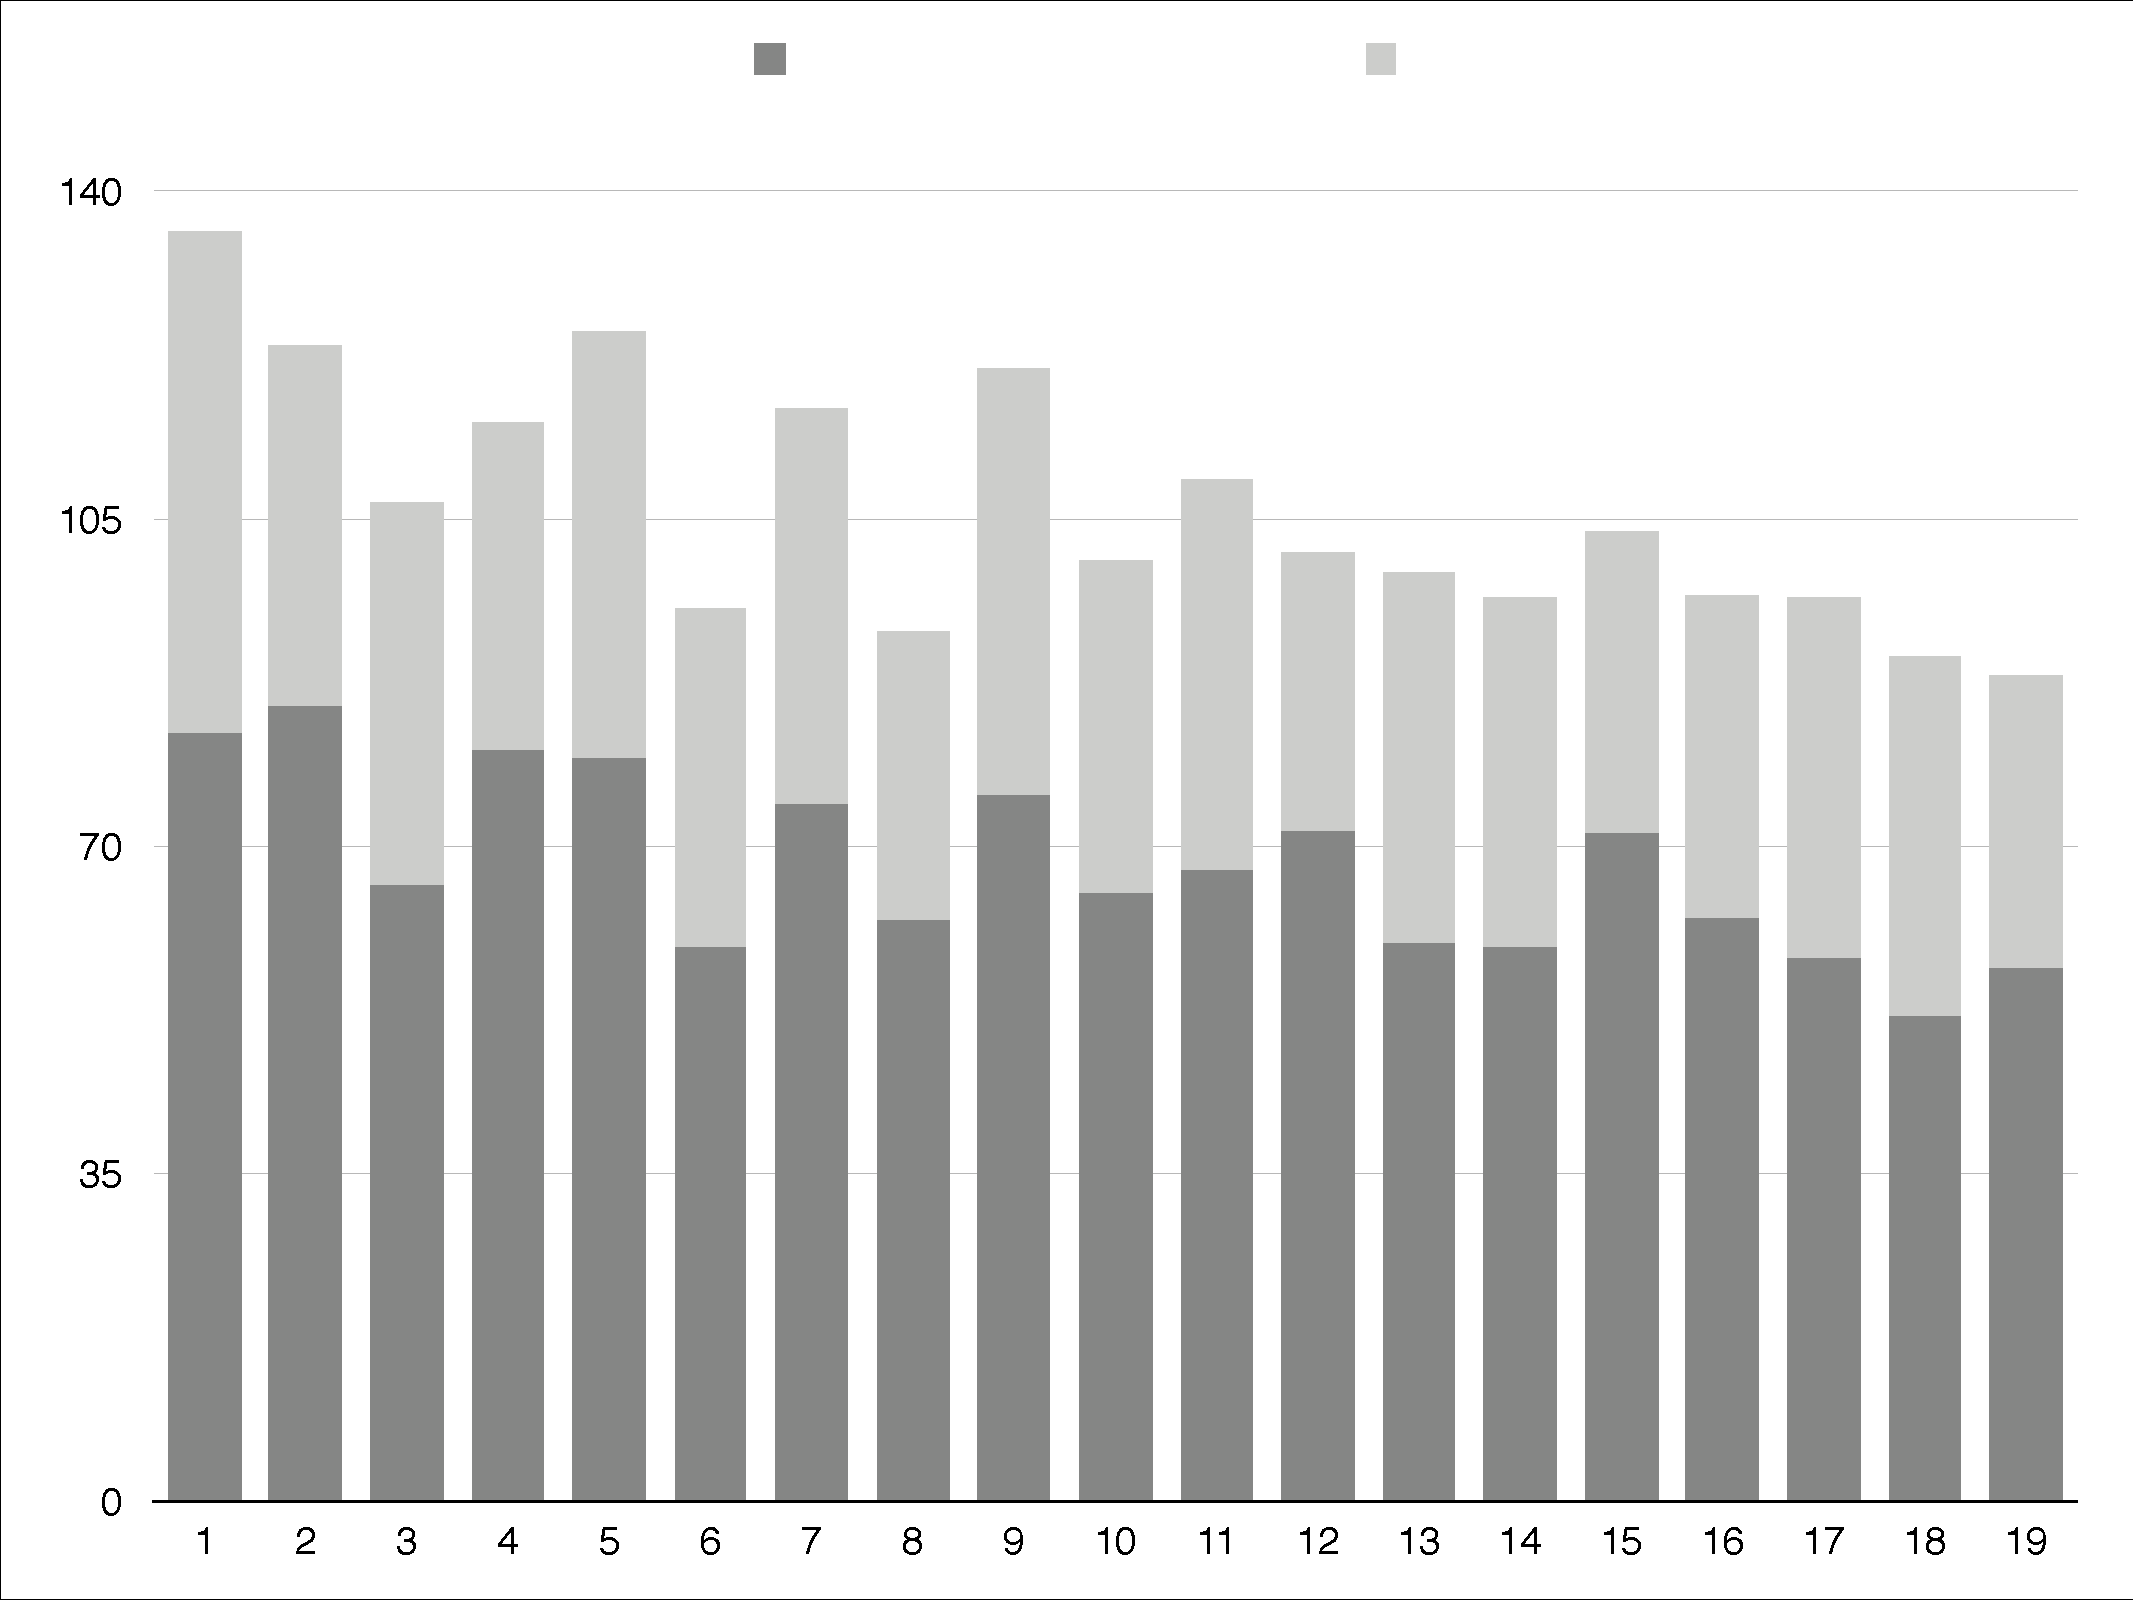
\includegraphics[width=\columnwidth]{OverheadDiagram.pdf}
\caption{\label{Fi:overhead}Overhead breakdown into tag propagation (dark grey) and Bayesian analysis at sink (pale grey), where horizontal (X) axis denotes the number of propagation steps and vertical (Y) axis denotes overhead}
\end{figure}

\OC{\paragraph{Accuracy} For accuracy comparison, we considered real-world benchmark applications.} These are listed in the first two columns of \tableref{realworld}. To select the apps, ensuring no biases, we applied the following methodology: We started from the 65 Google Play apps not chosen for the training phase. We then excluded 8 apps that do not have permission to access sensitive data and/or perform release operations (i.e., their manifest does not declare sufficient permissions out of {\tt INTERNET}, {\tt READ\_PHONE\_STATE}, {\tt SEND\_SMS}, etc), as well as 3 apps that we did not manage to install properly, resulting in 54 apps that installed successfully and exercise privacy sources and sinks.
 
We deployed the apps under the two \Tool\ configurations. Each execution was done from a clean starting state. 
The third column of \tableref{realworld} denotes whether our exploration of the app was exhaustive. By that we mean exercising all the UI points exposed by the app in a sensible order. Ideally we would do so for all apps. However, (i) some of the apps, and in particular gaming apps, had stability issues, and (ii) certain apps require SMS-validated sign in, which we did not perform. We did, however, create Facebook, Gmail and Dropbox accounts to log into apps that demand such information yet do not ask for SMS validation. We were also careful to execute the exact same crawling scenario under both the T-BD and H-BD configurations. We comment, from our experience, that most data leaks happen when an app launches, \OC{and initializes advertising/analytics functionality}, and so for apps for which deep crawling was not possible the results are still largely meaningful. 
 
The complete results are listed in \tableref{realworldAll}. The last eight columns of \tableref{realworld} summarize the findings by H-BD and T-BD, respectively, at the granularity of privacy items: the device number, Android and device identifiers, and location. 
%
%
The warnings reported by the H-BD configuration are available for review.\footnote{
	See archive file realworldapps.zip at \href{https://www.dropbox.com/sh/ggrcvqsbkiubmlb/faSUXmr9xK}{https://www.dropbox.com/sh/
	ggrcvqsbkiubmlb/faSUXmr9xK}.
}
%
We manually classified the findings into true positives (TPs) and false positive (FPs). For this classification, we scrutinized the reports by the two configurations, and also --- in cases of uncertainty --- decompiled and/or reran the app to examine its behavior more closely. 

\begin{figure*}
\begin{minipage}[b]{0.95\columnwidth}
\begin{lstlisting}
$\fbox{source : private value}$
    GeoCoder.getFromLocation(...) : [ Lat: ..., Long: ..., 
	    Alt: ..., Bearing: ..., ..., $\textbf{IL}$ ] 
	    
$\fbox{sink : arguments}$
  WebView.loadUrl(...) : http://linux.appwiz.com/
    profile/72/72_exitad.html?
    p1=RnVsbCtBbmRyb2lkK29uK0VtdWxhdG9y&
    p2=Y2RmMTUxMjRlYTRjN2FkNQ%3d%3d&
    ...    
    LOCATION=$\textbf{IL}$&
    ...
    MOBILE_COUNTRY_CODE=&
    NETWORK=WIFI
\end{lstlisting}
\caption{\label{Fi:ios7}Suppressed spurious leakage on {\tt ios7lockscreen}}
\end{minipage}
\hfill
\begin{minipage}[b]{0.95\columnwidth}
\begin{lstlisting}
$\fbox{source : private value}$
  Settings$\$$Secure.getString(...) : $\textbf{cdf15124ea4c7ad5}$
  
$\fbox{sink : arguments}$
  FileOutputStream.write(...) : 
    <?xml version='1.0' encoding='utf-8' 
    standalone='yes' 
    ?><map><string 
    name="openudid">$\textbf{cdf15124ea4c}$
\end{lstlisting}
\caption{\label{Fi:fruitninja}Suppressed spurious leakage on {\tt fruitninjafree}}
\end{minipage}
\end{figure*}

%For \Tool\ we report two numbers: The one in parentheses is the restriction of the findings to sources and sinks in common with TaintDroid, whereas the outer number counts all findings by \Tool. 

\begin{table*}
\begin{small}
\begin{center}
	\begin{tabular}{l|c|c|c|c|c|c|c|c|c|c}
	\multicolumn{1}{c|}{\multirow{2}{*}{App}} & \multicolumn{1}{c|}{\multirow{2}{*}{Domain}} & \multicolumn{1}{c|}{\multirow{2}{*}{Deep crawl?}} & \multicolumn{4}{c|}{H-BD} & \multicolumn{4}{c}{T-BD} \\
	\cline{4-11}
				& 																			  &   & no. & dev. ID          & And. ID     &    loc. &
 no. & dev. ID          & And. ID     &    loc. \\
	\hline
	{\tt at.nerbrothers.SuperJump}					& games/arcade 		& 		      				&
	             &     	&  		 \checkmark			& & & &    & \\
	{\tt atsoft.games.smgame}						& games/arcade & 	  \checkmark         & 
             &     \checkmark 	&  					& \checkmark & 
             &		\checkmark 	&  					& \checkmark \\
	{\tt com.antivirus}							& communication 			& 	     \checkmark      & 
             &     \checkmark 	&  					&  & 
            	&		\checkmark  & &    \\
	{\tt com.appershopper.ios7lockscreen}			& personalization 		& 	          & 
    \checkmark         &     \checkmark 	&  	\checkmark				& \checkmark &
    \checkmark  		& 		\checkmark &     \checkmark & \checkmark \\
    {\tt com.applicaster.il.hotvod}					& entertainment 		& \checkmark 	&
	             &     	&  		 \checkmark			& & 
	             &  &  \checkmark  & \\
    	{\tt com.bestcoolfungames.antsmasher}	& games/arcade 			&     \checkmark   & 
             &      	&  					& \checkmark &  
             & &    & \checkmark \\
     {\tt com.bigduckgames.flow}					& games/puzzles		& 		      		&
	             &     	&  		 \checkmark			& & & &    & \\
	{\tt com.bitfitlabs.fingerprint.lockscreen}			& games/casual 		& 	          & 
             &     \checkmark 	&  	\checkmark				&  & & &    & \\
             {\tt com.channel2.mobile.ui}					& news 				& \checkmark 	&
             	             &     	&  		 \checkmark			& &
	              & &  \checkmark  & \\
{\tt com.cleanmaster.mguard}					&  tools 				& 	    \checkmark       & 
             &     \checkmark 	&  	\checkmark				&  &
              & \checkmark  & \checkmark   & \\
	{\tt com.coolfish.cathairsalon}					&  games/casual 		& 	      \checkmark     & 
             &     \checkmark 	&  	\checkmark				&  & & &    & \\
	{\tt com.coolfish.snipershooting}				& games/action 		& 	  \checkmark         & 
             &     \checkmark 	&  	\checkmark				&  & & &    & \\
	{\tt com.cyworld.camera}						& photography  		& 		      		& 
		             &     	&  		 \checkmark			& & 
		             & &   \checkmark & \\
	{\tt com.devuni.flashlight} 					& tools 					& \checkmark   & 
		             &     	&  		 \checkmark			& & 
		            & 			& \checkmark   & \\
	{\tt com.digisoft.TransparentScreen}		& entertainment 			& 	     \checkmark      & 
             &      	&  	\checkmark				& \checkmark & 
             & 		&   \checkmark  				& \checkmark \\
             {\tt com.dropbox.android}						& productivity 			&\checkmark	&
                          	             &     	&  		 \checkmark			& & & &    & \\
{\tt com.g6677.android.cbaby}					& games/casual 		& 	          & 
             &     \checkmark 	&  	\checkmark				&  & & &    & \\
	{\tt com.g6677.android.chospital}				& games/casual 		& 	          & 
             &     \checkmark 	&  	\checkmark				&  & & &    & \\
  {\tt com.g6677.android.design}					& games/casual 		& 	          & 
             &     \checkmark 	&  			&  & & &    & \\
{\tt com.g6677.android.pnailspa}				& games/casual 		& 	          & 
             &     \checkmark 	&  	\checkmark				&  & & &    & \\
	{\tt com.g6677.android.princesshs} 				& games/casual 		& 	          & 
             &     \checkmark 	&  	\checkmark				&  & & &    & \\
{\tt com.goldtouch.mako}						& news 				& 	    \checkmark       & 
             &   \checkmark	  	&  				&  &
              &  \checkmark &    & \\
             {\tt com.goldtouch.ynet} 						& news 				& \checkmark 	&
             	             &     	&  		 \checkmark			& &
	             			 & & \checkmark   & \\
	   	{\tt com.google.android.youtube}				& media \& video		& 		      		& 
		     	             &     	&  		 \checkmark			& &
			              & &  \checkmark   & \\
	{\tt com.king.candycrushsaga}					& games/arcade 		& 		      		&
	   &     	&  		 \checkmark			& & & &    & \\
	{\tt com.skype.raider} 						& communication 			& 		      		&
	   &     	&  		 \checkmark			& &
	   & 		&    		\checkmark			& \\
	\hline \hline
	\multicolumn{1}{c|}{26} & & 13 & 1 & 13 & 21 & 4 & 1 & 5 & 10 & 4 \\
	\end{tabular}
	\end{center}
	\caption{\label{Ta:realworld}Findings due to the H-BD and T-BD \Tool\ configurations on 26/54 top-popular mobile apps (phone number abbreviated as no.; device 
	ID as dev. ID; Android ID as And. ID;  and location as loc.)}
\end{small}
\end{table*} 

\paragraph{Discussion} As \tableref{realworld} indicates, and \tableref{realworldAll} affirms more explicitly, the H-BD variant is more effective than the T-BD variant overall. \OC{Runtime overhead is lowered, and at the same time findings by H-BD are more complete, both in number of illegitimate leaks and in leakage types. This is mainly because of (i) the intrusive instrumentation required for tag propagation, which can cause instabilities, and (ii) inability to track tags through native code. (Both are discussed in detail in \appendixref{completeRes}.)}
At the same time, the loss in accuracy due to heuristic identification of relevant values is negligible, as suggested by the discussion in \secref{points}. H-BD triggers only one false alarm, on {\tt iso7lockscreen},
which is due to overlap between irrelevant values: extra information on the {\tt Location} object returned by a call to {\tt LocationManager.getLastKnownLocation(...)} and unrelated metadata passed into a {\tt ContextWrapper.startService(...)} request.  Finally, as expected, H-BD does not incur false negatives.

To give the reader a taste of the findings, we present in \figrefs{ios7}{fruitninja} two examples of potential leakages that \Tool\ (both the H-BD and the T-BD configurations) deemed legitimate. The instance in \figref{ios7} reflects the common scenario of obtaining the current (or last known) location, converting it into one or more addresses, and then releasing only the country or zip code. In the second instance, in \figref{fruitninja}, the 64-bit Android ID --- generated when the user first sets up the device --- is read via a call to \texttt{Settings$\$$Secure.getString(ANDROID\_ID)}. At the release point, into the file system, only a prefix of the Android ID consisting of the first 12 digits is published.   


%In the following, we discuss the accuracy, coverage and robustness trends that emerge from \tableref{realworld}.
%
%\paragraph{Accuracy} First, \Tool\ produces more complete results, triggering $>$x2.5 more alarms (21 vs 8) on $>$x2 of the benchmarks (15 vs 7) when restricted to the APIs supported by TaintDroid, and $>$x8 alarms (65 vs 8) on $\sim$x4 of the benchmarks (26 vs 7) in general. The results by both tools are highly precise. We identified only one false alarm --- by \Tool --- due to overlap between benign values: extra information on the {\tt Location} object returned by a call to {\tt LocationManager.getLastKnownLocation(...)} and unrelated metadata passed into a {\tt ContextWrapper.startService(...)} request. 
%
%There are no findings reported by TaintDroid that \Tool\ fails to detect. There are, however, alarms triggered by \Tool\ over source/sink pairs supported by TaintDroid that TaintDroid misses
%(e.g., on {\tt ios7lockscreen}, {\tt fingerprint} and {\tt princesshs}). We invested considerable time investigating into these findings, including decompiling the subject apps. For some of the apps (like {\tt princesshs}), the reason for the misses by TaintDroid appears to be that 
%TaintDroid limits loading of third-party libraries, and thus certain functionality is not executed, also leading to exceptional app states, which both inhibit certain data leaks.\footnote{
%	See \href{https://groups.google.com/forum/\#!topic/android-security-discuss/U1fteEX26bk}{forum comment} on this by William Enck, the TaintDroid moderator.
%} As for the remaining apps, these all leak data via the {\tt mobileCore} module,\footnote{ 
%\href{https://www.mobilecore.com/sdk/}{https://www.mobilecore.com/sdk/}
%} which is a highly optimized and obfuscated library, and so a plausible explanation for the misses is that data flow breaks within this library, though we could not confirm this. 
%
%A pleasing property of the data-centric approach, especially in comparison with taint analysis, is that it can record not only true alarms but also candidate leakages falling below the designated similarity threshold. We thus went through an extended log of our system, containing also suppressed alarms, and confirmed that all the source/sink pairs that the system resolved not to report were indeed benign. 
%
%\paragraph{Coverage} Our second observation is that the TaintDroid APIs are insufficient. The additional internet, system-settings and file-system APIs monitored by our system disclose many more data leaks. We expect that extending TaintDroid to include these additional APIs while retaining the same level of precision would not be easy. (See section 8 in \cite{EGCCJMS:OSDI10}.) We also anticipate observable impact on the performance of TaintDroid.
%
%\paragraph{Robustness} A final point is that \Tool\ appears more stable than TaintDroid, crashing on 8 of the 54 applications, which are a strict --- and small --- subset of the 21 apps TaintDroid crashes on. \Tool\ crashes all stem from missing libraries and/or hardware capabilities in the emulated environment. We conjecture that additional TaintDroid crashes are due to (i) TaintDroid restrictions on loading of third-party libraries, as well as (ii) the intrusive nature of the TaintDroid instrumentation scheme, which reaches into the lowest levels of the Android platform, thereby affecting its stability. This analysis suggests that our approach is more readily applicable to real-world applications.
%
%
%
%
%The tainting approach has been investigated, and shown to be feasible, across multiple studies. A notable implementation of the tainting approach is the TaintDroid system~\cite{EGCCJMS:OSDI10}. TaintDroid is the product of careful engineering, balancing between precision and performance to achieve admissible runtime overhead (mostly below 10\%). TaintDroid tracks taint labels across a select set of sources and sinks. It supports system-wide analysis by tainting files and interprocess messages. TaintDroid has been extended by, and used in, multiple recent studies~\cite{JHW:SPSM12,RCE:CODAPSY13,SPKS:WISTP12}.

\section{Related Work}\label{Se:related}

As most of the research on privacy monitoring builds on the tainting approach, we survey related research mainly in this space. We also mention several specific studies in other areas.

\paragraph{Realtime Techniques} The state-of-the-art system for realtime privacy monitoring is TaintDroid~\cite{EGCCJMS:OSDI10}. TaintDroid features tolerable runtime overhead of about 10\%, and can track taint flow not only through variables and methods but also through files and messages passed between apps. TaintDroid has been used, extended and customized by several follow-up research projects. Jung et al.~\cite{JHW:SPSM12} enhance TaintDroid to track additional sources (including contacts, camera, microphone, etc). They used the enhanced version in a field study, which revealed 129 of the 223 apps they studied as vulnerable. 30 out of 257 alarms were judged as false positives. The Kynoid system~\cite{SPKS:WISTP12} extends TaintDroid with user-defined security policies, which include e.g. temporal constraints on data processing as well as restrictions on destinations to which data is released.

The main difference between \Tool\ and the approaches above, which all apply information-flow tracking, is that \Tool\ exercises ``fuzzy'' reasoning, in the form of statistical classification, rather than enforcing a clear-cut criterion. As part of this, \Tool\ factors into the privacy judgment the data values flowing into the sink statement, which provides additional evidence beyond data flow.

\paragraph{Quantitative Approaches} Different approaches have been proposed for quantitative information-flow analysis, all unified by the observation that data leakage is a quantitative rather than boolean judgment. McCamant and Ernst~\cite{ME:PLDI08} present an offline dynamic analysis that measures the amount of secret information that can be inferred from a program's outputs, where the text of the program is considered public. Their approach relies on taint analysis at the bit level. It provides a sound upper bound on the actual information flow, but only with respect to the observed runs.
Newsome et al.~\cite{NMS:PLAS09} develop complementary techniques to bound a program's \emph{channel capacity} using decision procedures (SAT and \#SAT solvers). They apply these techniques to the problem of false positives in dynamic taint analysis. Backes et al.~\cite{BKR:SP09} measure leakage in terms of indistinguishability, or equivalence, between outputs due to different secret artifacts. Their characterization of equivalence relations builds on the information-theoretic notion of entropy.
Budi et al.~\cite{BLJL:PLDI11} propose $kb$-anonymity, a model inspired by $k$-anonymity for ensuring safe release of private data for the purposes of testing and debugging. Like $k$-anonymity, $kb$-anonymity replaces certain information in the original data for privacy preservation, but beyond that, it also ensures that the replaced data does not lead to divergent program behaviors, and thus testing and debugging are still effective.

While these proposals have all been shown useful, none of these approaches has been shown to be efficient enough to meet realtime constraints. The algorithmic complexity of computing the information-theoretic measures introduced by these works seriously limits their applicability in a realtime setting. Our approach, instead, enables a quantitative/probabilistic mode of reasoning that is simultaneously lightweight, and therefore acceptable for online monitoring, by focusing on relevant features that are efficiently computable.

\paragraph{Static and Hybrid Analysis} The PiOS tool~\cite{EKKV:NDSS11} performs static leakage analysis of iOS applications. PiOS combines backward slicing with forward constant propagation for accurate resolution of method calls. It then performs standard taint analysis atop the resulting call graph, where path length is (unsoundly) limited to a maximum of 100 basic blocks. The authors report that over half of the 1,400 apps they analyzed leak the unique ID of their host device.
Graa et al.~\cite{GCCC:CSS12} propose a hybrid tainting technique that augments dynamic taint analysis with certain classes of implicit flows (namely, those due to conditional statements). To do so, they apply intraprocedural static analysis to the control flow graph of a method at load time to detect variable assignments that occur only under one conditional branch. The FlowDroid tool~\cite{FARBBKTOM:TR13} performs static leakage analysis of Android applications using tainting. It accounts for the Android lifecycle model, handles callbacks and features flow, field and object sensitivity. FlowDroid builds on, and extends, previous taint analyses designed for the server side~\cite{TPFSW:PLDI09,TPCCG:FASE13} as well as client side~\cite{GPTDTB:ISSTA11} of web applications.

In our experience, even precise static analysis techniques often suffer from a large number of false findings. These are due both to the qualitative (and coarse) nature of taint analysis and to other approximations (e.g., call-graph imprecisions). As for hybrid techniques, current techniques address challenges like implicit flows, where our experience suggests that for effective detection of data leakage by authentic apps, a more important dimension is the form and quantity of released information. In \secref{conclusion}, we outline a hybrid variant of \Tool\ that we plan to develop.

\paragraph{Offline Algorithms} The AppsPlayground framework~\cite{RCE:CODASPY13}, built atop TaintDroid, performs dynamic analysis of mobile apps. It features automatic triggering of system events, including usage of contextual information to provide meaningful textual input. The AdRisk system~\cite{GZJS:SPWMN12} identifies potential privacy and security risks due to embedded in-app advertisement libraries. It first decouples the embedded ad libraries from the host app, and then applies state analysis to each of the libraries to approximate its behavior. 
AdSplit~\cite{SDW:SEC12} handles third-party advertising services differently by recompiling the app to extract such services, which consequently run as separate processes under separate user IDs. 

Our approach is extensible to the offline setting, e.g. by piggybacking on unit/integration tests and detecting leakage bugs during the development and testing phases of a mobile app. Our technique can also be integrated with frameworks like AppsPlayground, which provide automated crawling capabilities, to perform offline testing for leakage vulnerabilities.
\section{Conclusion and Future Work}\label{Se:conclusion}

In this paper, we articulated the problem of privacy enforcement in mobile systems as a classification problem. The traditional approach of information-flow tracking then becomes a ``binary'' classifier, which equates data leakage with source/sink data flow. We explored an alternative approach based on statistical classification, which addresses more effectively the inherent fuzziness in leakage judgements, accounting beyond data flow also for the amount and form of private information about to be released. We have instantiated our approach as the \Tool\ system, which is about to be featured in a commercial security product. Our experimental data establishes the high accuracy of \Tool\ as well as its applicability to real-world mobile apps.

Moving forward, we have two main objectives. The first is to extend \Tool\ with additional feature types. Specifically, we would like to account for (i) sink properties, such as file access modes (private vs public), the target URL of HTTP communication (same domain or third party), etc; as well as (ii) the history of privacy-relevant API invocations up to the release point (checking e.g. if/which declassification operations were invoked). Our second objective is to optimize our flow-based method for detecting relevant values (see \secref{featext}) by applying (offline) static taint analysis to the subject program, e.g. using the FlowDroid tool~\cite{FARBBKTOM:TR13}.  

\bibliographystyle{plain}
\bibliography{paper}

\newpage

\appendix

\section{Detailed Results on Real-world Apps}\label{Se:completeRes}

In \secref{practical}, we describe an experiment designed to evaluate our Bayesian analysis in ``pure'' form, i.e. without the support of information-flow tracking to detect relevant values. To make our description of this experiment complete, we include \tableref{realworldAll}, which provides a detailed summary of the results of this experiment across all benchmarks (including ones on which no leakages were detected).
%
For comparability between the H-BD and T-BD configurations, we count different dynamic reports involving the same pair of source/sink APIs as a single leakage instance.

\begin{table*}
\begin{small}
\begin{center}
	\begin{tabular}{l|c|c|c|c}
	\multicolumn{1}{c|}{App} & Domain & Deep crawl? & H-BD & T-BD \\
	\hline
	{\tt air.au.com.metro.DumbWaysToDie}			& games/casual 		& 		      		& 0 (C) & 0 (C) \\
	{\tt at.nerbrothers.SuperJump}					& games/arcade 		& 		      		& 1 & 0 (C) \\
	{\tt atsoft.games.smgame}						& games/arcade 		& \checkmark 	& 6 & 6  \\
	{\tt com.antivirus}							& communication 			& \checkmark 	& 1 & 1 \\
	{\tt com.appershopper.ios7lockscreen}			& personalization 		&		      		& 8 (1 FP) & 7 \\
	{\tt com.applicaster.il.hotvod}					& entertainment 		& \checkmark 	& 2 & 2 \\
	{\tt com.appstar.callrecorder}					& tools 					& 		      		& 0        & 0    \\
	{\tt com.awesomecargames.mountainclimbrace\_1}						
											& games/racing					& 		      		& 0 (C) & 0 (C) \\
	{\tt com.bestcoolfungames.antsmasher}	& games/arcade 			& \checkmark 	& 2 & 2 \\
	{\tt com.bigduckgames.flow}					& games/puzzles		& 		      		& 2 & 0 (C) \\
	{\tt com.bitfitlabs.fingerprint.lockscreen}			& games/casual 		& 		      		& 4 & 0 \\
	{\tt com.channel2.mobile.ui}					& news 				& \checkmark 	& 2 & 2  \\
	{\tt com.chillingo.parkingmaniafree.android.rowgplay} 		
													&	 games/racing 		& 				& 0 (C) & 0 (C) \\
	{\tt com.cleanmaster.mguard}					&  tools 				&\checkmark	& 2 & 2 \\
	{\tt com.coolfish.cathairsalon}					&  games/casual 		&\checkmark	& 5 & 0 (C) \\
	{\tt com.coolfish.snipershooting}				& games/action 		&\checkmark	& 5 & 0 (C) \\
	{\tt com.cube.gdpc.isr}						& health \& fitness 			& 				& 0 (C) & 0 (C) \\
	{\tt com.cyworld.camera}						& photography  		& 		      		& 1 & 1 \\
	{\tt com.devuni.flashlight} 					& tools 					& \checkmark   		& 2 & 2 \\
	{\tt com.digisoft.TransparentScreen}		& entertainment 			&\checkmark	& 2 & 2 \\
	{\tt com.domobile.applock}					& tools  					&\checkmark	& 0 & 0   \\
	{\tt com.dropbox.android}						& productivity 			&\checkmark	& 1 & 0 (C) \\
	{\tt com.ea.game.fifa14\_row}					& games/sports 		& 		      		& 0 & 0 (C) \\
	{\tt com.ebay.mobile}							& shopping 				& 					& 0 & 0 \\
	{\tt com.facebook.katana} 						& social 				& \checkmark 	& 0 & 0 \\
	{\tt com.facebook.orca} 						& communication 		& 	     			& 0  & 0 \\
	{\tt com.g6677.android.cbaby}					& games/casual 		& 				& 2    & 0 (C) \\
	{\tt com.g6677.android.chospital}				& games/casual 		& 		      		& 2 & 0 (C) \\
    {\tt com.g6677.android.design}					& games/casual 		& 		      		& 2 & 0 (C) \\
	{\tt com.g6677.android.pnailspa}				& games/casual 		& 		      		& 2 & 0 (C) \\
	{\tt com.g6677.android.princesshs} 				& games/casual 		& 		      		& 2 & 0 (C) \\
	{\tt com.gameclassic.towerblock}				& games/puzzles 		&\checkmark	& 0 & 0 (C) \\
	{\tt com.gameloft.android.ANMP.GloftDMHM}		& games/casual 	&		      		& 0  & 0   \\
	{\tt com.game.fruitlegendsaga}					& games/puzzles 		& 		      		& 0 & 0 \\
	{\tt com.gau.go.launcherex}					& personalization 			& 		      		& 0 & 0 \\
	{\tt com.glu.deerhunt2}						& games/arcade 			& 				& 0 (C) & 0 (C) \\
	{\tt com.goldtouch.mako}						& news 				&\checkmark	& 3 & 3 \\
	{\tt com.goldtouch.ynet} 						& news 				& \checkmark 	& 2 & 2 \\
	{\tt com.google.android.apps.docs}				& productivity 			& 		      		& 0 & 0 \\
	{\tt com.google.android.apps.translate}			& tools 					& 		      		& 0 & 0 \\
	{\tt com.google.android.youtube}				& media \& video		& 		      		& 1 & 1 \\
	{\tt com.google.earth}						& travel \& local 			& 				& 0 (C) & 0 (C) \\
	{\tt com.halfbrick.fruitninjafree}					& games/arcade 		& 		      		& 0 & 0 \\
	{\tt com.halfbrick.jetpackjoyride}				& games/arcade 		&\checkmark	& 0 & 0 \\
	{\tt com.icloudzone.AsphaltMoto2}				& games/racing 		& 		      		& 0 & 0 \\
	{\tt com.ideomobile.hapoalim}					& finance 				& 		      		& 0 & 0 \\
	{\tt com.imangi.templerun2} 					& games/arcade 		& 		      		& 0 (C) & 0 (C) \\
	{\tt com.kiloo.subwaysurf} 						& games/arcade 		& 		      		& 0 (C) & 0 (C) \\
	{\tt com.king.candycrushsaga}					& games/arcade 		& 		      		& 1 & 0 (C) \\
	{\tt com.sgiggle.production}					& social 					& 		      		& 0       & 0     \\
	{\tt com.skype.raider} 						& communication 			& 		      		& 2 	& 2 \\
	{\tt com.UBI.A90.WW} 						& games/arcade 			& 		      		& 0        & 0   \\
	{\tt com.viber.voip} 							& communication 			&		      		& 0        & 0    \\
	{\tt com.whatsapp} 							& communication 			&		      		& 0        & 0   \\
	\hline \hline
	{\bf total / apps:}	& & 18 / 54  & 65 / 26 (1 FP)  & 35 / 14
	\end{tabular}
	\end{center}
	\caption{\label{Ta:realworldAll}Detailed summary of the results of the H2 experiment described in \secref{practical}}
\end{small}
\end{table*} 

Analogously to \tableref{realworld}, the first two columns of \tableref{realworldAll} list the applications and their respective domain, and the middle column denotes whether crawling was exhaustive. The last two columns specify the overall number of findings by the H-BD and T-BD variants, respectively. We also indicate whether at any point during the run we experienced runtime errors, crashes or abnormal behaviors using the ``(C)'' label alongside the number of findings.

As \tableref{realworldAll} highlights, the difference in leakage alarms by the H-BD and T-BD variants is dramatic. We have analyzed it, and came to the following explanations:
\begin{compactitem}
\item First, as noted in \secref{practical}, the T-BD variant introduces significantly more instability than the H-BD variant, causing illegal application behaviors in 21 cases (compared to only 8 under H-BD). We have investigated this large gap between the H-BD and T-BD configurations, including by decompiling the subject apps. Our analysis links the vast majority of illegal behaviors to limitations that
TaintDroid casts on loading of third-party libraries. For this reason, certain functionality is not executed, also leading to exceptional app states, which both inhibit certain data leaks.\footnote{
	For a technical explanation, see forum comment by William Enck, the TaintDroid moderator, at \href{https://groups.google.com/forum/\#!topic/android-security-discuss/U1fteEX26bk}{https://groups.google.com/forum/\#!topic/android-security-discuss/U1fteEX26bk}.
} 
\item A secondary reason why H-BD is able to detect more leakages, accounting for {\tt com.bitfitlabs.fingerprint.lockscreen}, is that this benchmark makes use of the {\tt mobileCore} module,\footnote{ 
\href{https://www.mobilecore.com/sdk/}{https://www.mobilecore.com/sdk/}
} which is a highly optimized and obfuscated library. We suspect that data flow breaks within this library, though we could not fully confirm this. 
\end{compactitem}



\end{document} 





